% Final report (architecture document), D7065E.
% Build with `make` in this directory: it renders ../diagrams/*.d2 into
% figures/ and compiles this file. The text is in sections/.
\PassOptionsToPackage{unicode}{hyperref}
\PassOptionsToPackage{hyphens}{url}
\PassOptionsToPackage{dvipsnames,svgnames,x11names}{xcolor}
\documentclass[11pt]{article}
\usepackage{amsmath,amssymb}
\usepackage{lmodern}
\usepackage{iftex}
\ifPDFTeX
  \usepackage[T1]{fontenc}
  \usepackage[utf8]{inputenc}
  \usepackage{textcomp}
\fi
\IfFileExists{microtype.sty}{\usepackage[]{microtype}\UseMicrotypeSet[protrusion]{basicmath}}{}
\usepackage{parskip}
\usepackage{xcolor}
\IfFileExists{xurl.sty}{\usepackage{xurl}}{}
\usepackage{bookmark}
\hypersetup{
  pdftitle={Energy-Aware Ventilation and Climate Control: Architecture Document},
  pdfauthor={Kasper Axelsson, Mohamd Amar Chms Aldden},
  colorlinks=true,
  linkcolor={RoyalBlue},
  filecolor={Maroon},
  citecolor={Blue},
  urlcolor={Blue}}
\urlstyle{same}
\usepackage[a4paper,margin=2.4cm]{geometry}
\usepackage{longtable,booktabs,array}
\usepackage{calc}
\usepackage{graphicx}
\usepackage{caption}
\captionsetup{font=small,labelfont=bf,skip=6pt}
\usepackage{float}
\usepackage{fancyvrb}
\setlength{\emergencystretch}{3em}
\providecommand{\tightlist}{\setlength{\itemsep}{0pt}\setlength{\parskip}{0pt}}
\setcounter{secnumdepth}{-\maxdimen}
\usepackage{newunicodechar}
\newunicodechar{°}{\textdegree}
\newunicodechar{₂}{\textsubscript{2}}
\newunicodechar{→}{\ensuremath{\rightarrow}}
\newunicodechar{≤}{\ensuremath{\leq}}
\newunicodechar{≥}{\ensuremath{\geq}}
\newunicodechar{≈}{\ensuremath{\approx}}
\newunicodechar{×}{\ensuremath{\times}}
\newunicodechar{✓}{\ensuremath{\checkmark}}
\newunicodechar{–}{--}
\newunicodechar{—}{---}
\usepackage{etoolbox}
\AtBeginEnvironment{longtable}{\footnotesize}
\AtBeginEnvironment{tabular}{\footnotesize}
\usepackage{fancyhdr}
\pagestyle{fancy}\fancyhf{}
\rhead{\small D7065E\,--\,Architecture Document}
\lhead{\small Energy-Aware Ventilation \& Climate Control}
\cfoot{\thepage}
\renewcommand{\headrulewidth}{0.4pt}
\usepackage{titlesec}
\titleformat{\section}{\Large\bfseries}{\thesection}{0.6em}{}
\titleformat{\subsection}{\large\bfseries}{\thesubsection}{0.5em}{}
\titleformat{\subsubsection}{\normalsize\bfseries}{\thesubsubsection}{0.5em}{}
\usepackage{pgfplots}
\pgfplotsset{compat=1.16}

% --- helpers ----------------------------------------------------------------
\newcommand{\COtwo}{CO\textsubscript{2}}
\newcommand{\code}[1]{\texttt{#1}}
\newcolumntype{L}[1]{>{\raggedright\arraybackslash}p{#1}}
% Something the authors still have to do. Every \todo must be gone before
% submission: `grep -n '\\todo' sections/*.tex report.tex`.
\definecolor{todored}{RGB}{176,0,32}
\newcommand{\todo}[1]{\par\noindent{\setlength{\fboxsep}{5pt}%
  \fcolorbox{todored}{todored!6}{\parbox{\dimexpr\linewidth-2\fboxsep-2\fboxrule}{%
  \small\textcolor{todored}{\textbf{To do before submission.}} #1}}}\par\vspace{0.4em}}
% A figure that does not exist yet.
\newcommand{\missingfigure}[1]{\par\begin{center}\fcolorbox{todored}{todored!6}{%
  \parbox[c][2.4cm][c]{0.82\linewidth}{\centering\small\textcolor{todored}{\textbf{Missing figure.}} #1}}\end{center}\par}
\DefineVerbatimEnvironment{json}{Verbatim}{fontsize=\footnotesize,xleftmargin=1em}
% ---------------------------------------------------------------------------

\begin{document}

\begin{center}
{\LARGE Energy-Aware Ventilation \& Climate Control\par}
\vspace{0.5em}
{\large D7065E, Architecture Document\par}
\vspace{1em}
{Kasper Axelsson \& Mohamd Amar Chms Aldden\par}
\vspace{0.3em}
{\small Draft of 10 October 2026\par}
\end{center}

\todo{This is a first full draft, written from \code{docs/*.md} and the code as
of commit \code{e9b01be}. Read every section against what you built. Open
points, each also marked where it belongs:
(1) the dashboard screenshots (Section 12);
(2) a response-over-time plot from the evaluation runs (Section 11);
(3) the tests with no recorded run: T-10, T-14, T-15, T-21, T-23, T-31, and
the larger-building part of T-22 (Section 10);
(4) the requirement priorities in Section 3, which are proposed, not decided;
(5) two requirements whose stated criterion is \emph{not} met, FR-4 and the
second half of NFR-3: decide how to word them (Sections 3, 10 and 11);
(6) the demo scenario in Section 2;
(7) the version and date in Section 1.}

\vspace{0.6em}

{
\hypersetup{linkcolor=black}
\setcounter{tocdepth}{2}
\tableofcontents
}

\section{1. Summary}

The system ventilates and heats 50 rooms of the LTU A-house, as modelled in
BuildSim, so that the air stays good while as little energy as possible is
spent on rooms nobody is in. Every room has a \COtwo{} sensor, a temperature
sensor and a people counter, a ventilation damper and a radiator valve; each of
these 250 devices is its own process. A controller decides the airflow and the
heating setpoint for every room once per model minute, and can start
ventilating before people arrive, from an occupancy profile learned from stored
readings. BuildSim holds the shared building state; this project provides the
room physics, the devices, the control, the storage and the dashboard around
it.

One principle runs through the design: \textbf{the controller proposes, and
nothing depends on the controller being right.} The actuators enforce the
safety limits themselves, a room whose sensor or controller goes quiet falls
back to design airflow on its own, and the true state of the rooms never
reaches the controller, only what the sensors report. Whatever fails, the
failure is towards more air, not less.

\begin{longtable}[]{@{}L{0.26\linewidth}L{0.68\linewidth}@{}}
\toprule
\textbf{Field} & \textbf{Value} \\
\midrule
\endhead
\textbf{Project title} & Energy-Aware Ventilation \& Climate Control \\
\textbf{Team members} & Kasper Axelsson, Mohamd Amar Chms Aldden \\
\textbf{Use case} & Indoor air quality and thermal comfort at minimum energy \\
\textbf{Repository} & \url{https://github.com/MisterD0ctor/d7065e-project} \\
\textbf{Version / date} & Draft, commit \code{e9b01be} / 2026-10-10 \\
\bottomrule
\end{longtable}

\textbf{Changes since the proposal.} Each change below was forced by something
we measured or by a course rule we had missed. Their consequences are discussed
in Section 13.

\begin{longtable}[]{@{}L{0.25\linewidth}L{0.27\linewidth}L{0.40\linewidth}@{}}
\toprule
\textbf{The proposal said} & \textbf{Now} & \textbf{What forced it} \\
\midrule
\endhead
The controller never sees occupancy and estimates it from \COtwo{} alone &
Every room has a people counter, with noise and faults like any other sensor &
Time. The proposal named this as the fallback. The \COtwo{} mass balance it
wanted to invert survives as the check that finds a stuck counter (D-11) \\
We simulate the people ourselves &
The course's occupancysim, changed in two places: fixed 5-second steps and a
record of every room at every whole minute &
Two runs of the same day agreed in only 99.6--99.7~\% of samples, so the
oracle replayed a slightly different week. After the change they are
identical (T-25) \\
Sensors and actuators as two components &
One process per device, 250 of them, and a registry in which an installer
commissions each one &
Lecture 1 makes one process per sensor and actuator a pass/fail rule; the
lecturer suggested the installer's database \\
REST, with a broker if polling does not keep up &
MQTT for observations, decisions and events; REST polling of BuildSim kept as
the fallback &
Four consumers need the same readings: controller, damper override, storage
and dashboard \\
Safety is part of the controller &
The damper enforces the flow floors, the \COtwo{} override and the command TTL
itself &
An override that dies with the controller protects nothing (Lecture 1,
``independent, bounded override'') \\
Heating follows a schedule &
The schedule, with an optimal start before 07:00 &
The first evaluation: rooms at 17.9~°C at 07:00 and below 20~°C until 08:13 \\
Gradient boosting if a time-of-day profile is too blunt &
The profile stayed &
The profile is not what limits the forecast: lecture rooms have no pattern
to learn (Section 11). A larger model would not help; a timetable input would \\
A dashboard overlay on the 3D view &
The overlay, and our own page with graphs over time &
The viewer shows the building now; the questions asked of a ventilation system
are about how it got there \\
Evaluation over a simulated week &
Five simulated weekdays per policy, and a training week before them &
Weekends are empty, and four policies had to fit in a day of runs (NFR-8) \\
\bottomrule
\end{longtable}

\section{2. Use case and building context}

\textbf{The building.} BuildSim models the LTU A-house: three floors and 838
rooms, with a REST API for equipment, sensor values and actuator states, and a
3D viewer. It stores the current state only. It has no physics, no history, no
clock, and it comes back blank after a restart. We instrument 50 rooms on the
ground floor: the 3 fika rooms, 20 lecture rooms, 24 offices and 3 small rooms
that the people simulation never uses. They are a seeded random sample, listed
in \code{deploy/devices.csv}, so the set is the same in every run.

\textbf{The people.} occupancysim, a course example, generates each day from a
seed and the date: staff in their offices, fika breaks around 09:45 and 14:30,
lunch at 12:00--13:00, lectures in four fixed slots, and three guards on patrol
at night. It also owns the model clock, which runs 60 or 120 times faster than
real time in our runs. Every time and duration in this document is model time
unless it says ``real''.

\textbf{How our processes use BuildSim.} The devices write to BuildSim, and
only the devices:
\begin{itemize}
\tightlist
\item Each \textbf{sensor device} writes its reading
  (\code{PUT /api/sensors/\{id\}/value}).
\item Each \textbf{actuator device} writes the state it has reached
  (\code{PUT /api/actuators/\{id\}/state}).
\item \textbf{physics} reads the actuators' reached states from BuildSim and
  never writes to it.
\item The \textbf{registry} creates the equipment records, and recreates them
  when BuildSim restarts.
\item \textbf{viz} writes the room layers and alerts the viewer shows.
\end{itemize}
This differs from the report guide, which has the simulator write sensor values
into BuildSim and sensor processes read them back. We follow Lectures 1 and 2
instead: sensor processes produce the readings, and the true room state never
enters BuildSim or anything the controller can read. The course material
disagrees with itself here, and the lectures' version is the one that keeps the
truth out of the controller's reach.

\textbf{Actors.} The \emph{facility manager} watches air quality, energy and
alerts, in the 3D viewer and on our graphs page. The \emph{installer} mounts
devices and records each one's id, kind and room in the registry; a device does
nothing until that is done. \emph{Occupants} affect the system only by being in
a room. None of them is on the control path.

\textbf{Why the decision is not trivial.} Air quality and energy pull in
opposite directions, and a room answers slowly. Its \COtwo{} time constant is
the room volume divided by the airflow: about 12 minutes for a lecture room at
design flow, about an hour for an office, and about two hours for any room
while its damper sits at the occupied minimum. A controller that waits for the
\COtwo{} sensor to show that a room has filled is already behind. One that
knows the room is about to fill can open the damper early and gently. Whether
that is worth anything here is what the evaluation in Section 11 measures, by
comparing four policies over the same simulated week: constant design flow,
reactive control on measured \COtwo{}, our predictive policy, and an oracle
that knows the true future occupancy.

\textbf{Scenario for the demonstration.} On a weekday morning the fika room
1570 is empty and its \COtwo{} is at 417~ppm. At 09:28 the predictive policy
raises its airflow to 112~l/s for the 11 people the profile expects within the
room's lead time of 22 minutes; the break starts at about 09:45. Then a
\COtwo{} sensor is frozen: after five identical readings the controller stops
believing it, commands design flow, and the dashboard raises an alert. Finally
the controller is stopped: every damper's last command expires after 300
seconds and it returns to design flow on its own.

\todo{Confirm that this is the demo you will give, or replace it. The first two
steps have been run (2026-09-30 smoke test; T-36). The third, stopping the
controller, has no recorded run yet (T-10, T-23).}

\section{3. Requirements}

Each requirement has an ID, a priority (M~must, S~should, C~could), a criterion
that can be measured, and the tests of Section 10 that verify it. The design
decisions in Section 4.4 cite these IDs, and Section 10 says for each one
whether it was met. All times are model time.

\todo{The priorities are a proposal. Decide them together.}

\subsection{Functional}

\begin{longtable}[]{@{}L{0.07\linewidth}L{0.04\linewidth}L{0.66\linewidth}L{0.13\linewidth}@{}}
\toprule
\textbf{ID} & \textbf{Pri} & \textbf{Requirement and acceptance criterion} & \textbf{Verified by} \\
\midrule
\endhead
FR-1 & M & Physics simulates \COtwo{} (mass balance) and temperature (heat
balance) per room, driven by the true occupancy and by the airflow and setpoint
the actuators have reached. A step response matches the analytic time constant
within 5~\%; a clock jump of hours gives no overshoot. & T-01, T-02 \\
FR-2 & M & Each room has a \COtwo{} sensor, a temperature sensor and a people
counter. Each samples its room every 60~s and reports with noise: \COtwo{}
±(30~ppm + 3~\%), temperature ±0.3~°C, count ±1. A fault (stuck, dropout,
drift) can be injected into one sensor without touching the others. & T-03, T-04 \\
FR-3 & M & The controller sets the airflow and the heating setpoint of every
room once per control period (60~s), and the next readings reflect it: the loop
closes. & T-05 \\
FR-4 & M & The controller forecasts each room's occupancy one lead time ahead
(the room's \COtwo{} time constant, 10--30~min) from a model trained offline on
stored sensor readings. On held-out days its error is lower than that of ``same
as now''. & T-06, T-35 \\
FR-5 & M & An actuator validates every command before applying it: range,
unit, time to live, duplicates (idempotent on \code{cmd\_id}). It rejects an
invalid command with a reason and moves towards an accepted target at a fixed
rate. & T-07, T-08 \\
FR-6 & M & Safety, enforced in the damper independently of the controller:
\COtwo{} above 1100~ppm gives maximum airflow whatever the command says, and
the flow never drops below 0.35~l/s·m² in occupied hours or 0.10~l/s·m²
otherwise. & T-09, T-10, T-11 \\
FR-7 & S & Degraded mode. A sensor that is silent for more than 3 samples, or
stuck on one value, is not acted on: a bad \COtwo{} sensor means design flow, a
bad temperature sensor 21~°C, a bad counter means the forecast and \COtwo{}
only. A stuck \COtwo{} sensor is found within 5 samples, a stuck temperature
sensor within 12, a stuck counter once the room's \COtwo{} contradicts it. The
decision names the mode and the fault. & T-12, T-13, T-36 to T-38 \\
FR-8 & M & Every observation, true room state, decision and actuator event is
stored with its model time and a run id, and a run's stored records are enough
to rebuild its results. & T-14 \\
FR-9 & M & The policy is chosen by one setting: \code{constant},
\code{reactive}, \code{predictive} or \code{oracle}. Nothing else differs
between two evaluation runs. & T-15, T-32 \\
FR-10 & S & The dashboard shows, per room, measured \COtwo{}, people counted
and expected, airflow and temperature, with alerts for overrides, silent or
stuck sensors and actuators on fallback: now, in the BuildSim viewer, and over
time, up to a week back, on our own page. & T-16, T-39 \\
FR-11 & S & A device does nothing until an installer has registered its id,
kind and room. The registry rejects a room that is not in the floor plan, and
keeps BuildSim's equipment list in step with what is installed, also after a
BuildSim restart. & T-17, T-28 to T-31 \\
\bottomrule
\end{longtable}

\subsection{Non-functional}

\begin{longtable}[]{@{}L{0.07\linewidth}L{0.04\linewidth}L{0.66\linewidth}L{0.13\linewidth}@{}}
\toprule
\textbf{ID} & \textbf{Pri} & \textbf{Requirement and acceptance criterion} & \textbf{Verified by} \\
\midrule
\endhead
NFR-1 & M & \textbf{Air quality.} \COtwo{} is at or below 1000~ppm in at least
95~\% of occupied room-minutes over five simulated weekdays
(\code{predictive}). & T-18 \\
NFR-2 & M & \textbf{Comfort.} The temperature is within 20--24~°C in at least
95~\% of occupied room-minutes. & T-19 \\
NFR-3 & S & \textbf{Energy.} The energy proxy (fans, heating of supply air,
radiators) of \code{predictive} is at least 30~\% below \code{constant}, and
no higher than \code{reactive} while meeting NFR-1 better than
\code{reactive} does. & T-20 \\
NFR-4 & S & \textbf{Latency.} A command shows up in BuildSim within one
control period (60~s, which is 1~s real at factor 60); reported as the 95th
percentile. & T-21 \\
NFR-5 & S & \textbf{Scale.} With 50 rooms (150 sensor writes per sample,
which is 150 per real second at factor 60), a full sample cycle finishes
within one sample period. & T-22 \\
NFR-6 & M & \textbf{Robustness.} Any one of our containers can be killed and
restarted without an unsafe state: a damper without valid commands returns to
design flow, and the loop resumes within 30~s real. & T-13, T-17, T-23, T-24 \\
NFR-7 & M & \textbf{Reproducibility.} The same seed and date give the same
occupancy in every room at every minute, and every number in this report
traces to a run id. & T-25 \\
NFR-8 & C & \textbf{Evaluation cost.} One policy over five simulated weekdays
runs in at most 2.5~h real. & T-26 \\
\bottomrule
\end{longtable}

Where the numbers come from. 1000~ppm is the usual indoor-air guideline. The
band 20--24~°C is the heating-season comfort range of EN~16798-1 category~II.
The airflows come from the Swedish workplace rule and the building code
(Section 6). NFR-3 is relative on purpose: the proposal treated the gap between
reactive control and the oracle as a result to report, not as a target.

\section{4. Architecture}

In every diagram an arrow points the way the data flows and is labelled with
what flows and the protocol. A two-way arrow says which way each part goes.

\subsection{4.1 Context diagram (C4 Level 1)}

\begin{figure}[H]
\centering
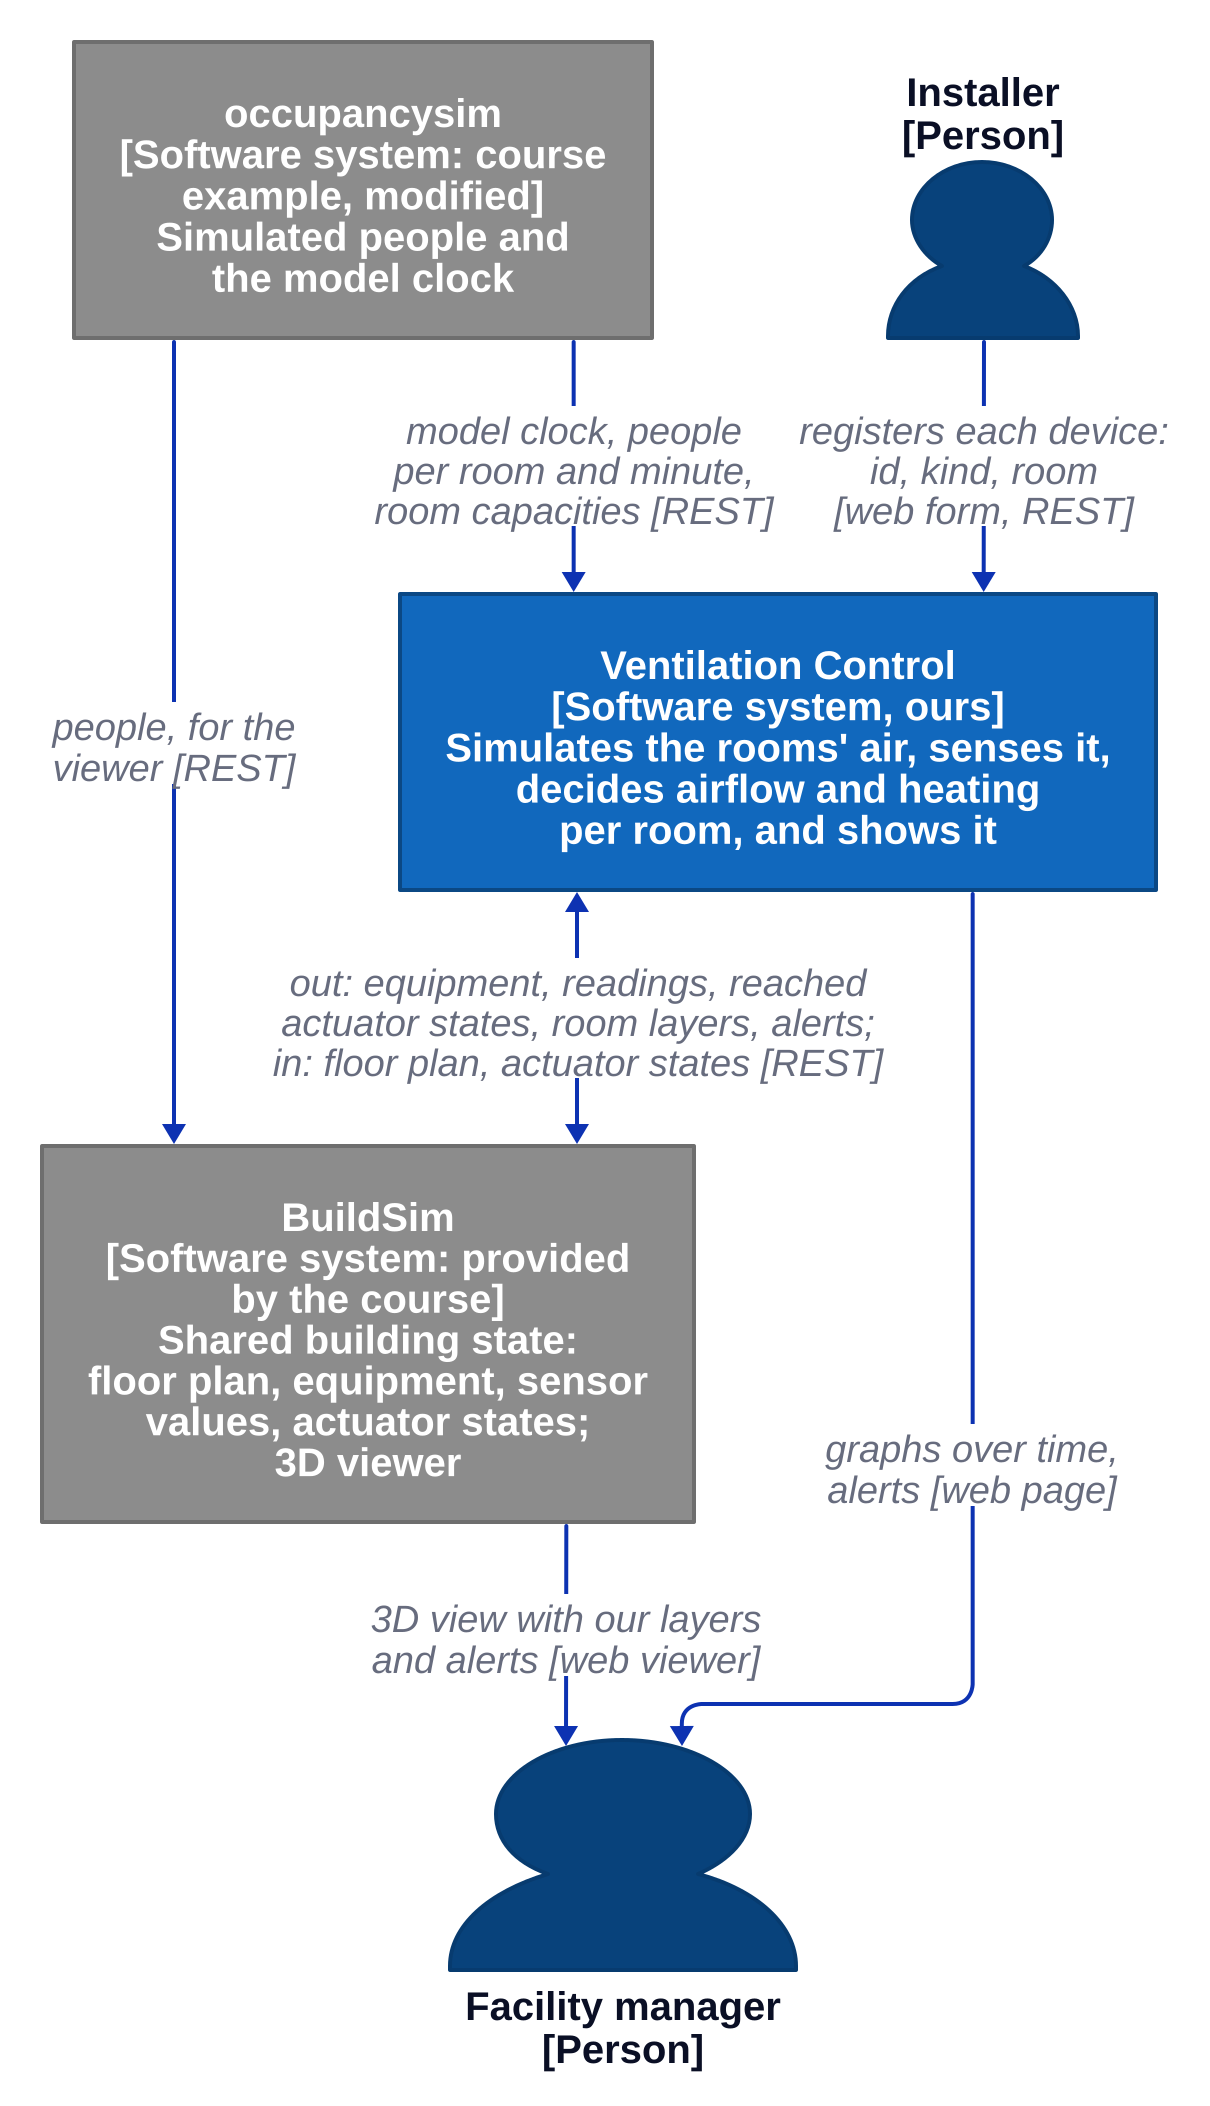
\includegraphics[width=0.52\linewidth]{figures/context.png}
\caption{System context. Our system is the blue box; the two grey systems come
from the course.}
\label{fig:context}
\end{figure}

\textbf{The boundary.} Everything we built is inside \emph{Ventilation
Control}, including the simulated room physics and the simulated devices. In a
real building those two would be the building itself and bought hardware; here
they are ours to write, and they are kept apart from the control side by the
truth boundary described in Section 4.2. \emph{BuildSim} is provided
infrastructure that we do not modify. \emph{occupancysim} is a course example
that we use as the source of people and of the model clock; we changed it in
two places (Section 6) and list the changes in \code{external/README.md}.

\textbf{The interactions.} The installer tells the system which device is in
which room. occupancysim supplies the clock and who is in each room at each
minute. Our system writes equipment, sensor readings, reached actuator states,
room layers and alerts to BuildSim, and reads the floor plan and the actuator
states back. The facility manager looks at the result in two places: BuildSim's
3D viewer, which shows the building now, and our own page, which shows it over
time.

\subsection{4.2 Container diagram (C4 Level 2)}

The container level is drawn as two views, because every link in one picture
is too dense to read on a page. Figure~\ref{fig:container} is the control loop
and the data path. Figure~\ref{fig:container-support} is commissioning and the
dashboard. Together they show every container and every link; the table after
them maps each box to its compose service and code folder.

\begin{figure}[H]
\centering
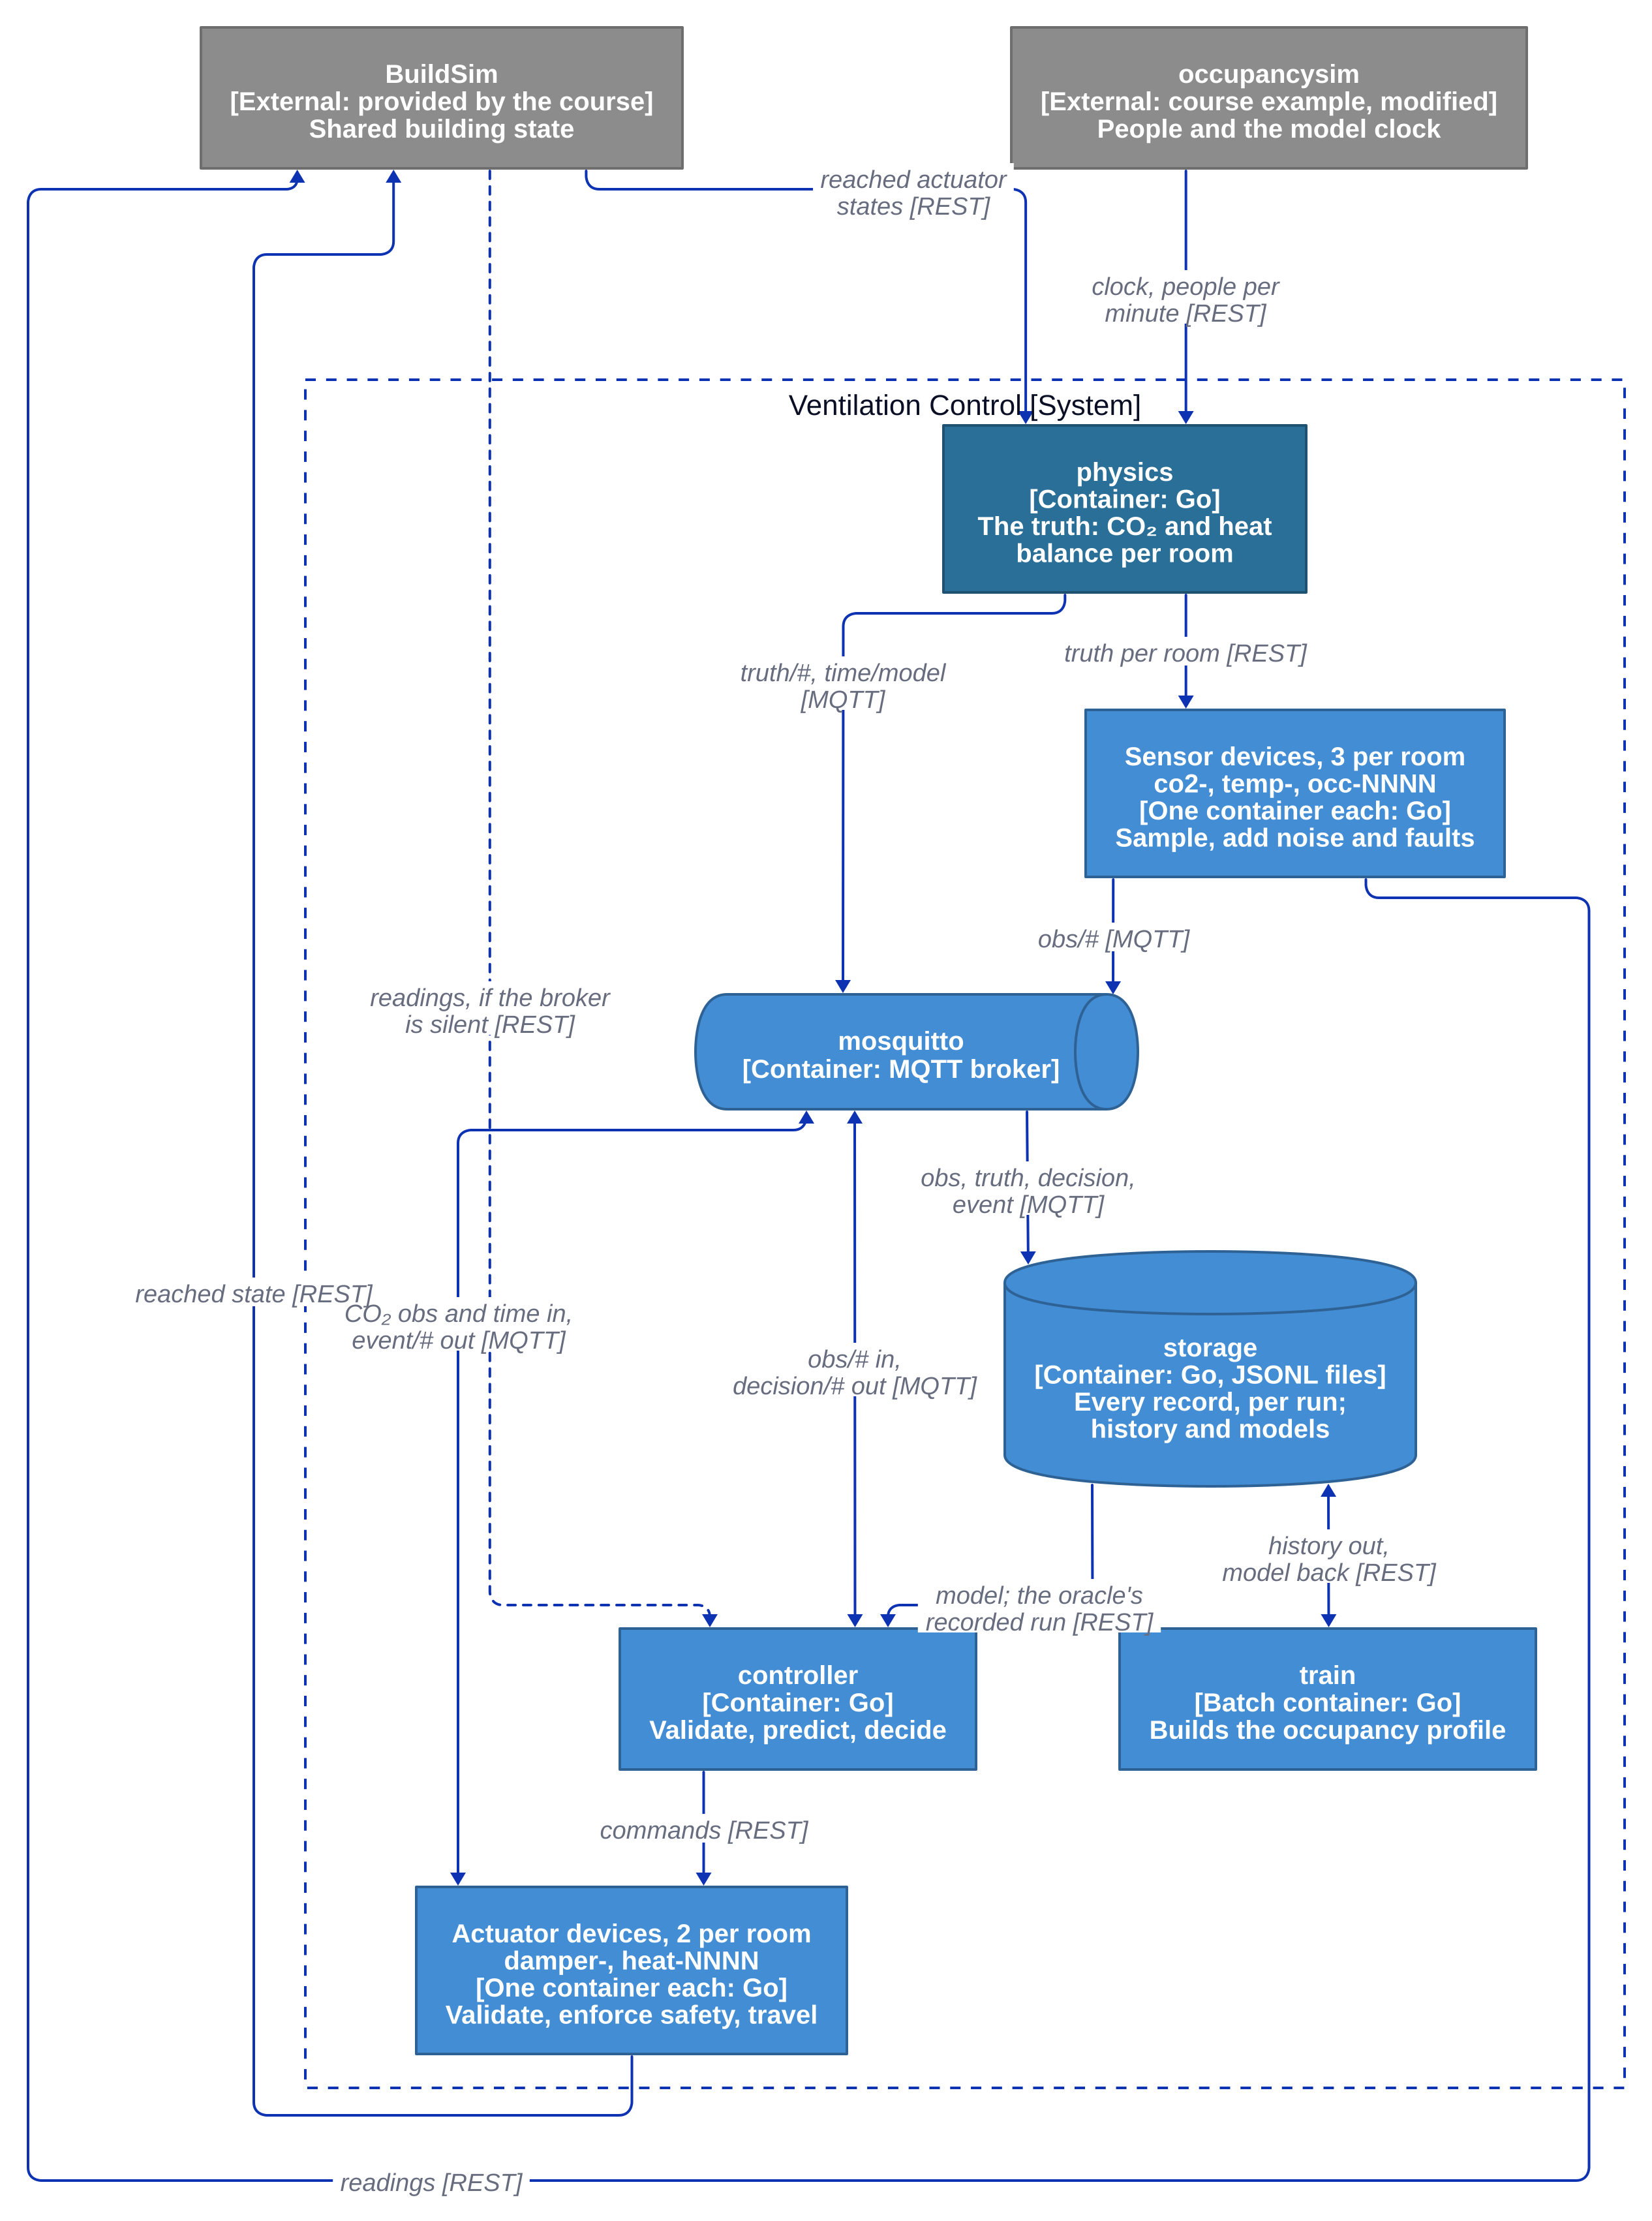
\includegraphics[height=0.78\textheight]{figures/container.png}
\caption{Containers, view 1: the control loop and the data path. One box is one
compose service, except the two device boxes, which are 150 and 100 containers.
The dashed arrow is the controller's fallback when the broker is silent; the
damper has the same fallback for its \COtwo{} reading.}
\label{fig:container}
\end{figure}

\begin{figure}[H]
\centering
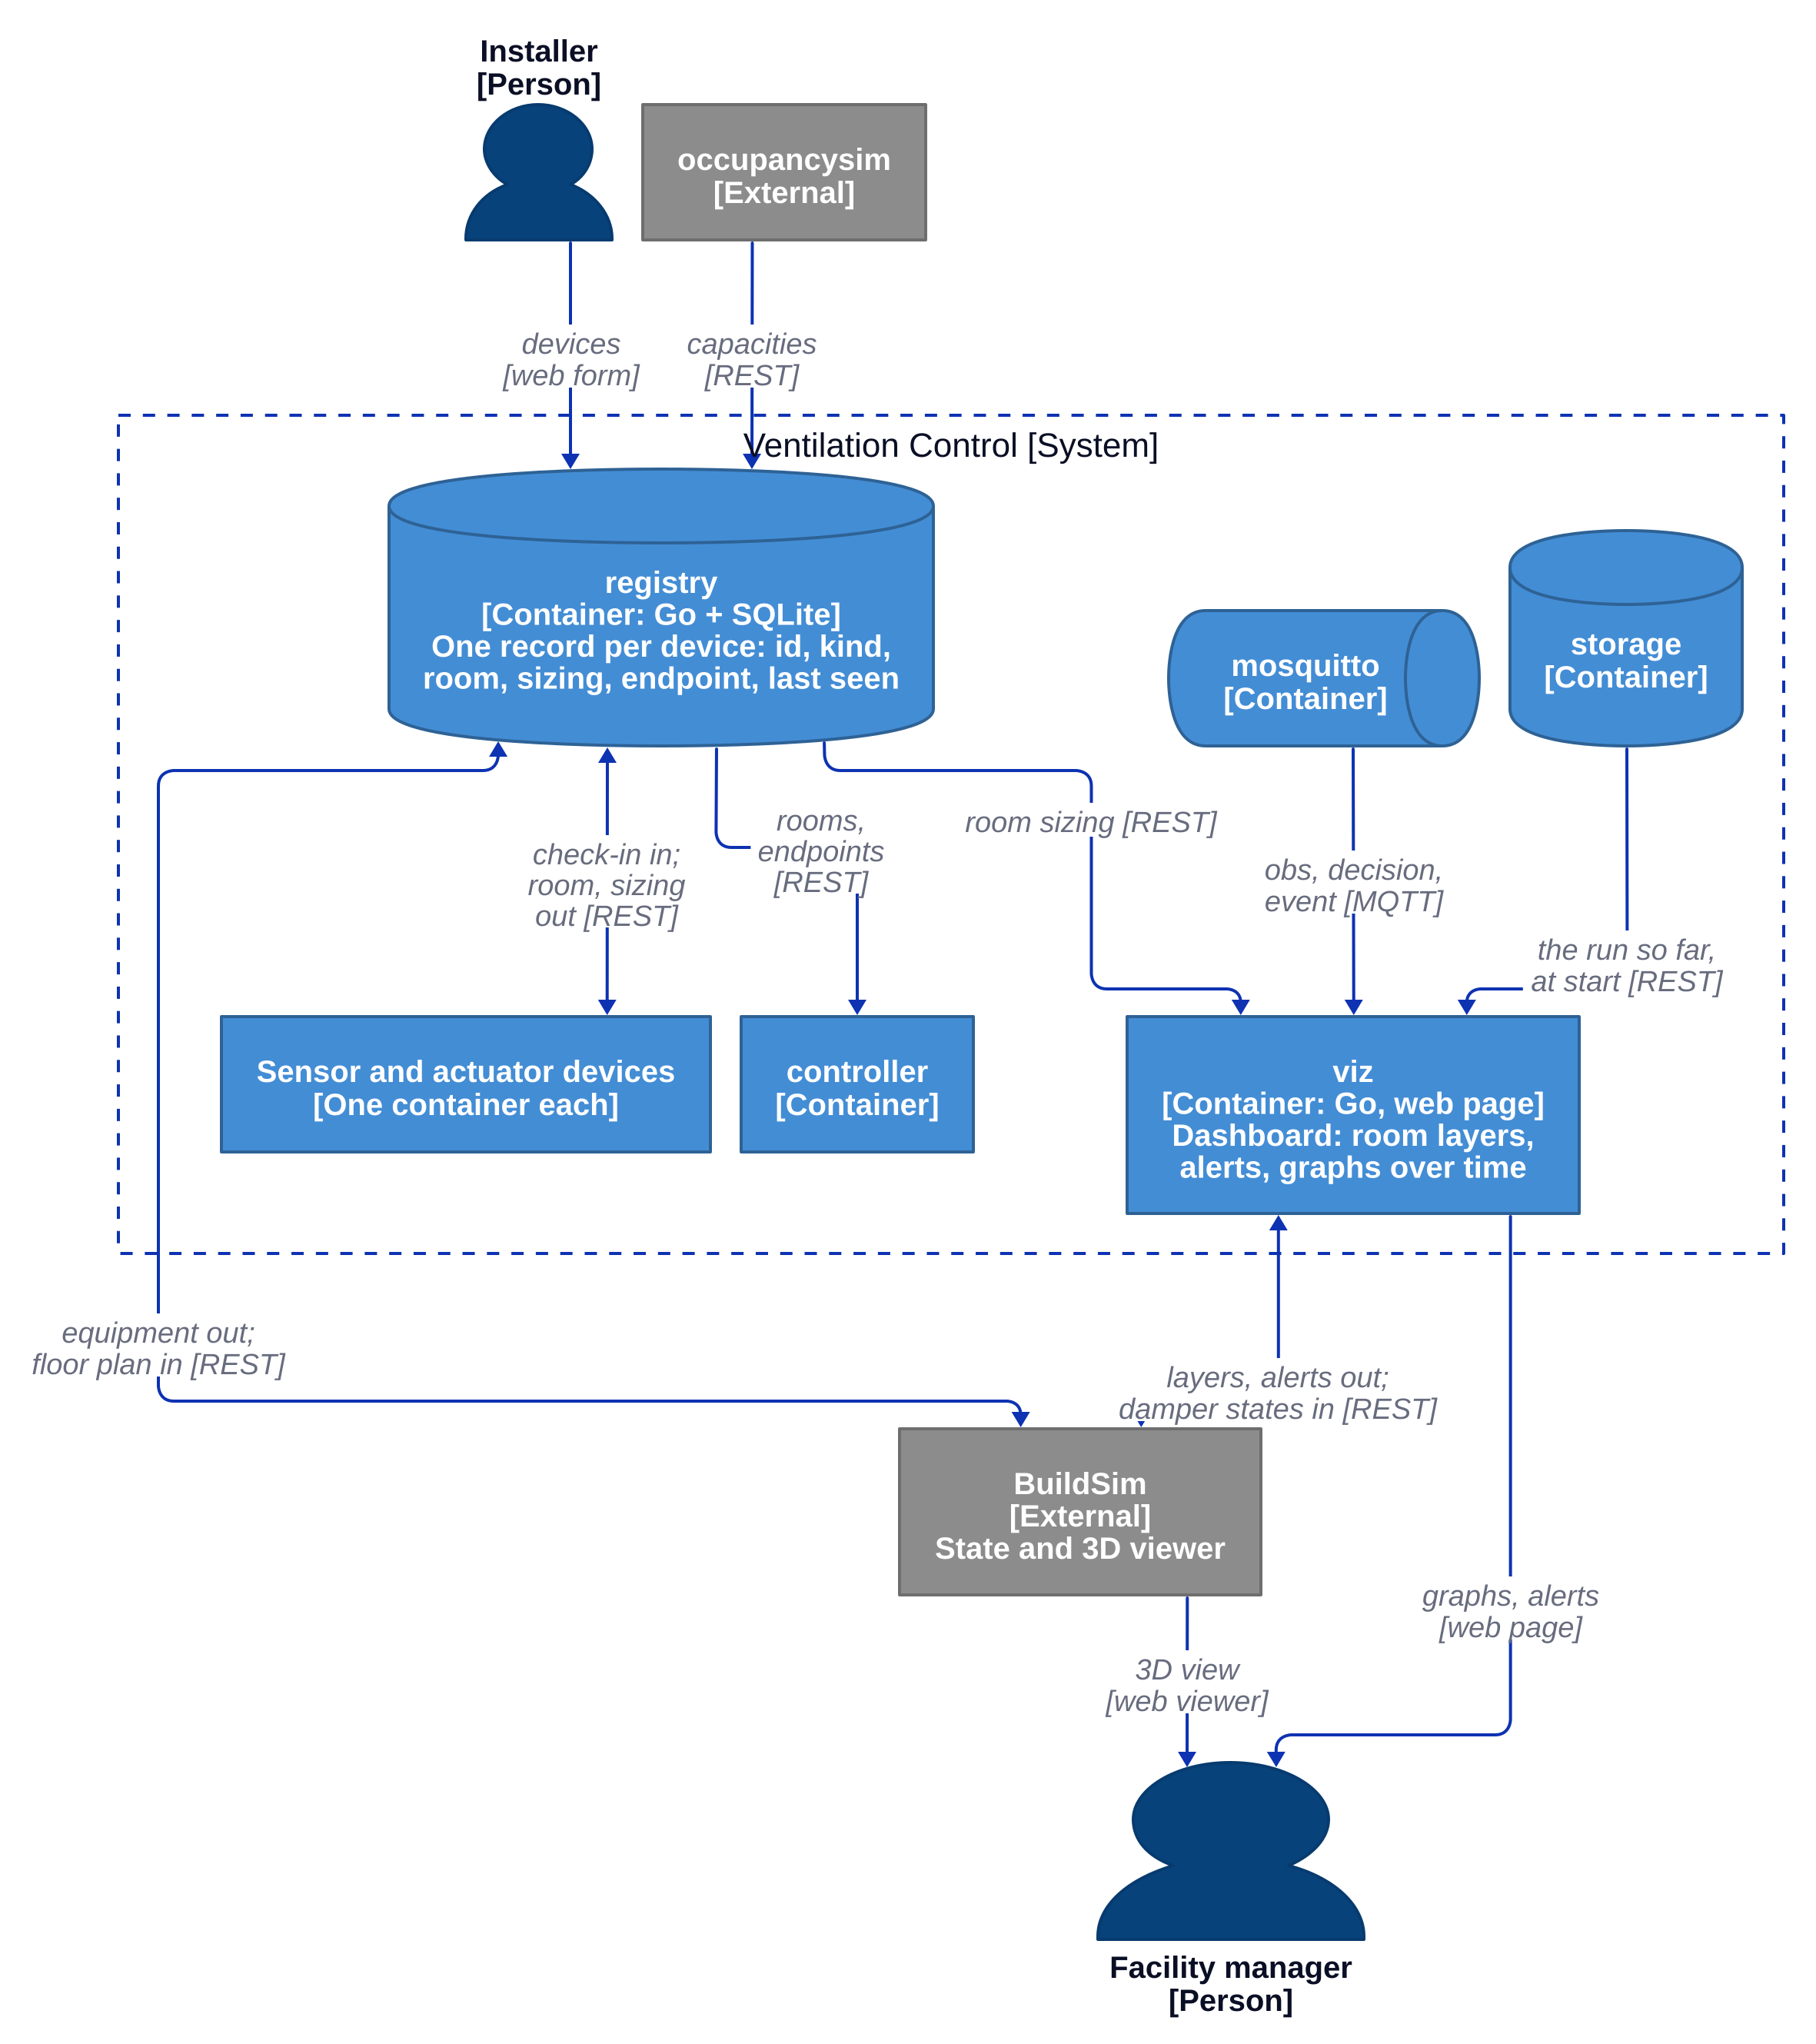
\includegraphics[width=0.74\linewidth]{figures/container-support.png}
\caption{Containers, view 2: commissioning (the registry) and the dashboard
(viz). The devices, the controller, the broker and storage are the same
containers as in Figure~\ref{fig:container}.}
\label{fig:container-support}
\end{figure}

\textbf{The loop.} physics computes each room's true \COtwo{} and temperature
from who is in the room (occupancysim) and from what the room's damper and
radiator valve have reached (read from BuildSim). Each sensor device samples
its own room's truth, adds noise, and reports the reading twice: to BuildSim,
which is the shared state the viewer shows, and to the broker, for everyone who
acts on it. The controller turns readings into commands and sends each command
to the actuator device it is meant for. The actuator validates it, applies the
safety limits, travels towards the target and writes the state it has reached
to BuildSim, where physics reads it. That last step closes the loop.

\textbf{The truth boundary.} Only three things know the true state of a room:
occupancysim, physics, and the sensor devices that sample it. The true state is
published on \code{truth/\#} for the evaluation, and the broker's access list
lets only storage read that topic. Storage in turn refuses to serve the truth
of the run that is in progress. The controller, the actuators and the dashboard
see sensor readings and nothing else. One part of the boundary is a convention
only: the controller shares the compose network with physics and could call its
truth API, although it has no code that does (Section 13).

\textbf{Why each container is its own process.} A network boundary is
justified when a part must be started, stopped, restarted or replaced on its
own. The right-hand column says what would be lost by merging.

\begin{longtable}[]{@{}L{0.14\linewidth}L{0.14\linewidth}L{0.30\linewidth}L{0.32\linewidth}@{}}
\toprule
\textbf{Compose service} & \textbf{Code} & \textbf{Its one job} & \textbf{Why a process of its own} \\
\midrule
\endhead
\code{physics} & \code{cmd/physics} & Compute every room's true state, one
model minute at a time & It is the building. Nothing on the control side may
share memory with it, or the truth leaks \\
\code{co2-NNNN}, \code{temp-NNNN}, \code{occ-NNNN} (150) & \code{cmd/sensor} &
Sample one room, add noise and faults, report & One device, one process, as in
a real installation: a dead sensor silences one room, and a fault is injected
into one device (FR-2, FR-7) \\
\code{damper-NNNN}, \code{heat-NNNN} (100) & \code{cmd/actuator} & Validate
commands, enforce the safety limits, travel, report & The override and the
fallback must work with the controller dead (FR-6, NFR-6) \\
\code{mosquitto} & \code{deploy/ mosquitto} & Carry observations, truth,
decisions, events and the model time & Decouples one publisher from four
consumers; enforces who may read the truth \\
\code{controller} & \code{cmd/controller} & Decide airflow and setpoint per
room & The part most likely to be wrong or replaced; the policy is swapped by
restarting it alone (FR-9) \\
\code{storage} & \code{cmd/storage} & Record every message per run; serve
history and models & Processes may share no files, so the files need one owner
with an API \\
\code{train} & \code{cmd/train} & Build the occupancy profile from stored
readings & Batch work, off the control path; run on demand \\
\code{registry} & \code{cmd/registry} & Know which device is installed where &
Outlives BuildSim restarts; devices and the controller find each other through
it \\
\code{viz} & \code{cmd/viz} & Show the building now and over time & A crashed
dashboard must not stop control \\
\bottomrule
\end{longtable}

The device containers are generated from the installation list:
\code{cmd/gendevices} writes \code{compose.devices.yaml} from
\code{deploy/devices.csv}. \code{cmd/install} and \code{cmd/evaluate} are tools
run by a person, not services.

\textbf{Communication patterns.} Three are used, each where it fits.
\emph{Publish/subscribe} (MQTT, QoS~1) carries the observations, because four
independent consumers need each reading: the controller, the damper's override,
storage and the dashboard. \emph{Request/response} (REST) carries commands,
because the controller needs to know at once whether a command was accepted,
clamped or refused; commands carry an id and a time to live, so a retry is
safe. \emph{Shared state} (BuildSim) is the fallback for both directions: when
the broker is silent, the controller and the dampers poll the readings there.
The model time is one retained MQTT message that physics refreshes every tick,
the way a building network distributes time to its devices.

\subsection{4.3 Component diagram (C4 Level 3): the controller}

\begin{figure}[H]
\centering
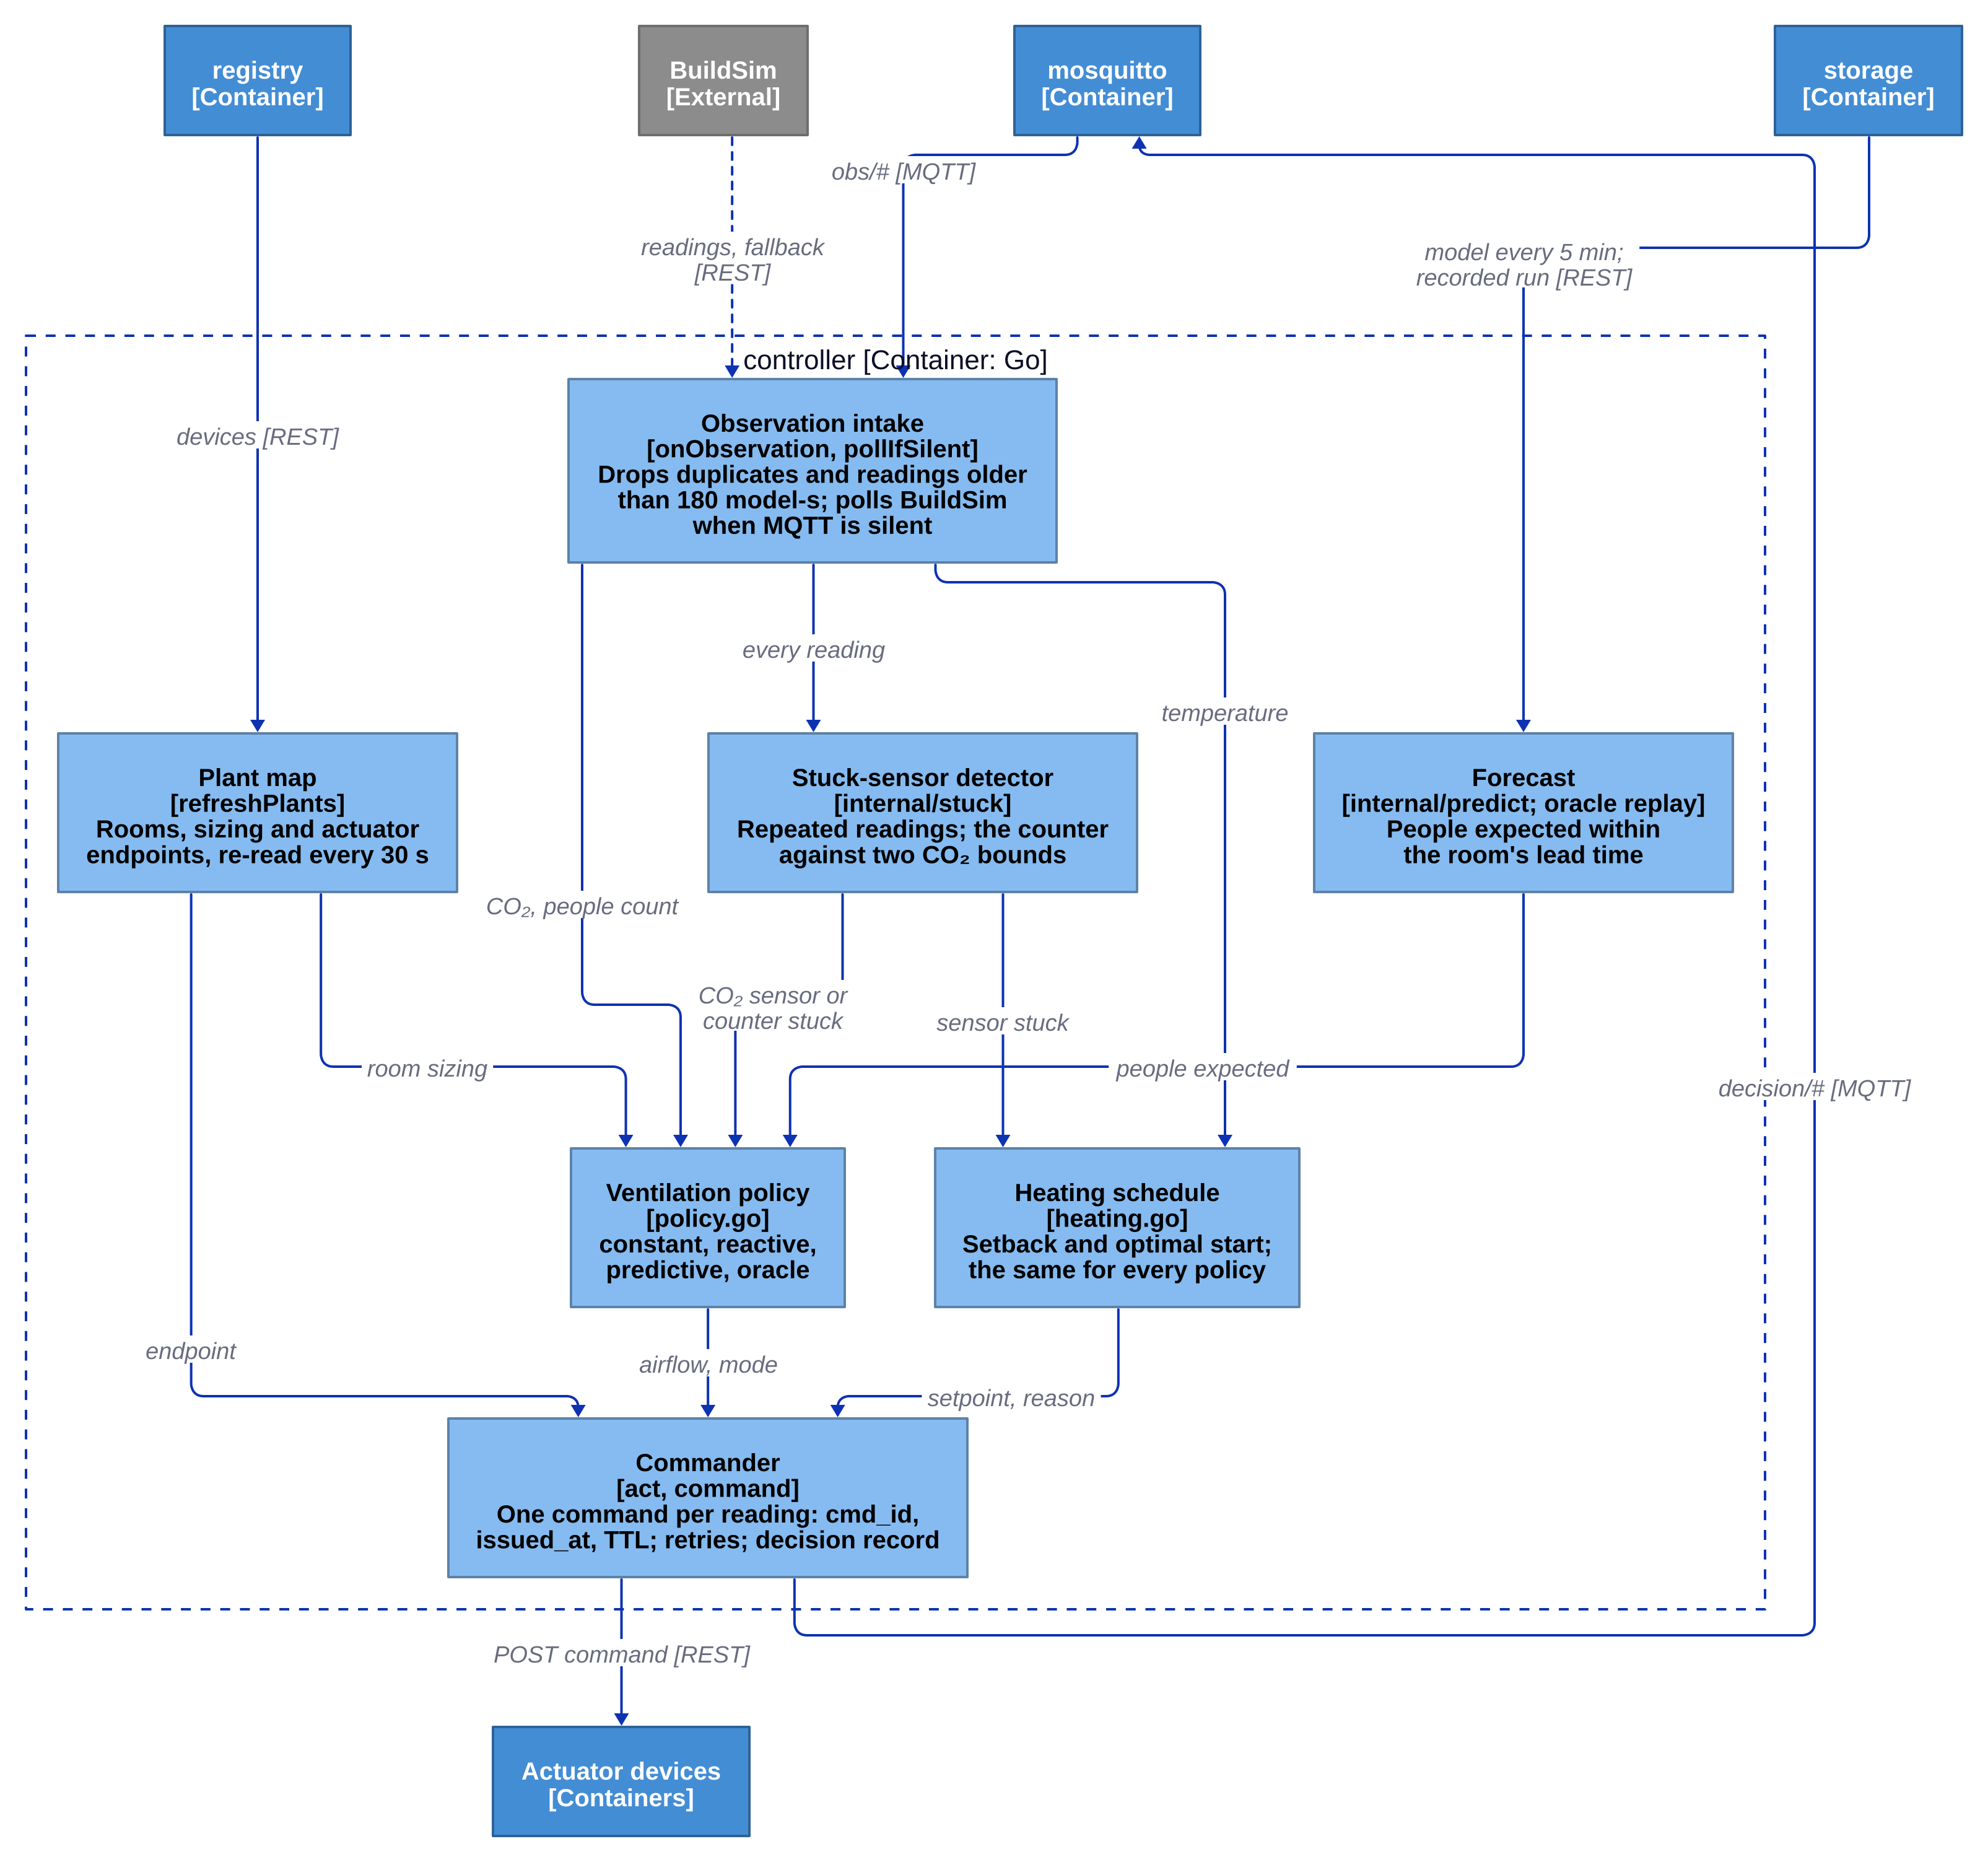
\includegraphics[width=0.92\linewidth]{figures/component.png}
\caption{Components of the controller. Each is a Go file or package in
\code{cmd/controller} and \code{internal/}.}
\label{fig:component}
\end{figure}

The controller makes one decision per reading. A \COtwo{} reading leads to an
airflow command for that room's damper, a temperature reading to a setpoint
command for its radiator valve, and a people count is remembered for the next
airflow decision. The \emph{observation intake} drops duplicates and readings
older than 180~s. The \emph{stuck-sensor detector} sees every reading and tells
the policy when a sensor's value can no longer be believed. The \emph{forecast}
answers one question, how many people to expect within the room's lead time,
either from the trained profile or, for the oracle, from the recorded truth of
an earlier run of the same dates. The \emph{ventilation policy} and the
\emph{heating schedule} are pure functions of those inputs. The
\emph{commander} sends the command, retries with the same id, and publishes the
decision record with what the actuator answered.

The split follows what changes independently. The four policies differ only in
the ventilation policy component, which is what makes the comparison in Section
11 fair. The forecast keeps the last model it loaded, so storage can be down
without the policy noticing.

\subsection{4.4 Design decisions and alternatives}

\begin{longtable}[]{@{}L{0.05\linewidth}L{0.24\linewidth}L{0.24\linewidth}L{0.07\linewidth}L{0.28\linewidth}@{}}
\toprule
\textbf{\#} & \textbf{Chosen} & \textbf{Alternatives rejected} & \textbf{Serves} & \textbf{Why, and the trade-off accepted} \\
\midrule
\endhead
D-1 & \textbf{Time.} Physics advances by whole model minutes from
occupancysim's per-minute record; every observation carries model time &
Each service keeps its own wall-clock × factor; physics samples BuildSim's
occupancy on its own tick & FR-1, NFR-7 & The second alternative is what we
built first: two runs of one day then disagreed in 0.3~\% of samples.
Trade-off: physics depends on an endpoint we added to occupancysim \\
D-2 & \textbf{Sensors.} One container per sensor device, sampling its room
from a truth API on physics & Physics writes noisy values to BuildSim itself;
one gateway per sensor kind & FR-2, FR-7 & The first breaks the one-process
rule and puts truth and observation in one process. The second, built first,
silences a whole kind when it crashes. Trade-off: 150 containers \\
D-3 & \textbf{Transport.} Sensors write to BuildSim and publish to MQTT;
consumers subscribe; BuildSim polling is the fallback & Everyone polls
BuildSim; a separate collector that polls and republishes & NFR-5, NFR-6 &
Four consumers need each reading. A collector adds a hop for data the sensor
already has. Trade-off: a broker to run, and two writes per reading that are
not atomic \\
D-4 & \textbf{Storage.} A storage service owns JSONL files per run and serves
them over HTTP & Files shared between logger, trainer and controller;
TimescaleDB & FR-8, NFR-7 & Shared files break a course rule. A database
server is hard to justify at 50 rooms. Trade-off: a history query reads the
whole run \\
D-5 & \textbf{Autonomy.} Validation, forecast and policy in one controller;
training as a batch job & The predictor as its own service & FR-3, FR-4 & No
network hop on the control path, and nothing else needs the forecast.
Trade-off: the parts cannot be restarted separately \\
D-6 & \textbf{Safety.} Enforced in the actuator: range, rate, TTL, flow
floors, \COtwo{} override & Inside the controller, after the policy; a
separate safety process & FR-5, FR-6, NFR-6 & It must survive a dead or wrong
controller. Trade-off: the damper needs the room's sizing and the \COtwo{}
stream, so it is no longer a plain device \\
D-7 & \textbf{Baselines.} One policy interface, four implementations; the
oracle replays the recorded truth of an earlier run of the same dates & An
oracle that reads occupancysim's plans & FR-9, NFR-7 & The oracle then uses
the same forecast interface as the predictor and never touches live truth.
Trade-off: it needs two runs of a day to be identical, which needed D-1 \\
D-8 & \textbf{Dashboard.} A viz process: layers and alerts in the BuildSim
viewer, and its own page of graphs & The viewer alone; Grafana over storage &
FR-10 & The viewer has no history. Grafana would need an index on our files
first. Trade-off: the graphs' history is a second copy, in viz's memory \\
D-9 & \textbf{Actuators.} One container per actuator device & One container
per kind for all rooms; one for everything & FR-5, NFR-6 & A failed damper
affects one room. Trade-off: 100 containers \\
D-10 & \textbf{Commissioning.} A registry with its own database; a device
learns its room at check-in & Device lists in configuration; registering
straight in BuildSim & FR-11 & BuildSim forgets everything on restart, and
configuration means nobody installs anything. Trade-off: one more service on
the start-up path, and devices do not authenticate \\
D-11 & \textbf{Stuck sensors.} A run of identical readings for \COtwo{} and
temperature; the counter against two \COtwo{} mass-balance bounds that hold
for any airflow & ``Counter unchanged while \COtwo{} moves''; estimating the
head-count from \COtwo{} and airflow & FR-7 & The first blames every healthy
counter when a lecture starts, because \COtwo{} lags the count. The second
needs the damper's true flow at every moment. Trade-off: blind to small
over-counts, and slow (15--75~min) \\
-- & \textbf{Room set.} 50 rooms on one floor, a fixed seeded sample & The
whole building (838 rooms); all of the floor (277) & NFR-5, NFR-8 & One
container per device makes the laptop the limit (Section 11). Trade-off: about
60~\% of the floor's lectures land in rooms we do not simulate \\
\bottomrule
\end{longtable}

Three of these were reversed by evidence, which is why their first versions
appear as rejected alternatives. D-1 and D-7: the oracle was designed on the
assumption that two runs of a day are identical, and the first evaluation
showed they were not. D-2 and D-9: gateways per kind were built first and
replaced by one process per device after the lecturer suggested an installer's device database. D-8: the viewer
alone was the first decision, and it could not answer how a room got to where
it is.

\section{5. Interfaces and data contracts}

% Long literal names in this section: let lines stretch instead of sticking out.
\sloppy

Each contract says what is sent, in which units, how often, when it counts as
stale, and what happens when the other side does not answer. The same
contracts, with every field, are kept next to the code in
\code{docs/interfaces.md}.

Conventions for every interface:
\begin{itemize}
\tightlist
\item \textbf{Rooms} are keyed \code{<level>/<room>}, for example
  \code{level0/A109}. Room names repeat between floors.
\item \textbf{Model time} is RFC~3339 as occupancysim's clock gives it, for
  example \code{2026-09-21T10:15:00Z}. Real time is used only for network
  timeouts.
\item \textbf{Run id.} Every process takes \code{RUN\_ID} from its environment
  and puts it in every record it publishes.
\item Values written to BuildSim are \textbf{strings} (BuildSim's rule). Values
  on MQTT and on our own HTTP APIs are JSON numbers.
\item MQTT is QoS~1, not retained except the model time, with a login per
  service. The broker's access list decides who may read and write each topic.
\end{itemize}

\begin{longtable}[]{@{}L{0.06\linewidth}L{0.30\linewidth}L{0.19\linewidth}L{0.24\linewidth}L{0.09\linewidth}@{}}
\toprule
\textbf{ID} & \textbf{Interface} & \textbf{Writer} & \textbf{Readers} & \textbf{Protocol} \\
\midrule
\endhead
IF-1 & Model clock, people per minute & occupancysim; physics relays the time & physics; actuators & REST, MQTT \\
IF-2 & Truth API & physics & sensor devices only & REST \\
IF-3 & Sensor readings in BuildSim & each sensor device & viewer; controller and damper as fallback & REST \\
IF-4 & Observations \code{obs/\ldots} & each sensor device & controller, dampers, storage, viz & MQTT \\
IF-5 & Truth \code{truth/\ldots} & physics & storage only & MQTT \\
IF-6 & Decisions \code{decision/\ldots} & controller & storage, viz & MQTT \\
IF-7 & Actuator events \code{event/\ldots} & actuator devices & storage, viz & MQTT \\
IF-8 & Actuator command & controller & one actuator device & REST \\
IF-9 & Actuator state in BuildSim & each actuator device & physics, viz, viewer & REST \\
IF-10 & Storage API & storage & controller, train, viz, people & REST \\
IF-11 & Room layers, alerts; graphs page & viz & viewer; a browser & REST \\
IF-12 & Device registry & registry & installer, devices, controller, viz & REST \\
\bottomrule
\end{longtable}

\subsection{The truth side}

\textbf{IF-1, clock and people.}
\code{GET occupancysim:8081/api/minutes?after=<time>} returns the clock and who
was in each room at every whole minute after \code{after}:

\begin{json}
{"clock": {"time": "2026-09-21T10:16:25Z", "factor": 120, "running": true},
 "minutes": [
  {"time": "2026-09-21T10:15:00Z", "rooms": {"level0/1570": {"occupants": 16}}},
  {"time": "2026-09-21T10:16:00Z", "rooms": {"level0/1570": {"occupants": 17, "guards": 1}}}]}
\end{json}

\code{occupants} counts everyone; \code{guards} says how many of them are night
guards. Empty rooms are left out. The last 240 minutes are kept. Physics asks
every 250~ms real. A paused clock gives no new minutes, so physics does not
step; it never extrapolates. On a timeout (500~ms) physics keeps its state and
asks again; the minutes it missed are still in the record. Physics also
publishes the time as a retained message on \code{time/model}
(\code{\{"model\_time": \ldots, "factor": 60\}}) every tick, which is where the
actuators take it from.

\textbf{IF-2, truth API.} \code{GET physics:8080/rooms?room=level0/A109}
returns \code{\{"run\_id", "model\_time", "rooms": \{"level0/A109":
\{"co2\_ppm": 612.4, "temp\_c": 21.3, "occupancy": 6\}\}\}}. Units: ppm, °C,
persons. \code{model\_time} is the whole minute the values belong to. A sensor
polls every 250~ms real and takes a reading when \code{model\_time} has
advanced by its sample period. On a timeout (500~ms) it publishes nothing, so
it goes silent downstream, which is what a dead device looks like.

\textbf{IF-5, truth topic} \code{truth/<level>/<room>}, one record per room and
model minute, readable by storage only:

\begin{json}
{"run_id": "eval-reactive-v2", "room": "level0/A109",
 "model_time": "2026-09-21T10:15:00Z",
 "co2_ppm": 612.4, "temp_c": 21.3, "occupancy": 6, "guards": 0,
 "airflow_ls": 180.0, "setpoint_c": 21.0,
 "fan_w": 270.0, "ahu_heat_w": 2160.0, "radiator_w": 310.0}
\end{json}

The three powers are averages over the minute that ended at \code{model\_time}
and are what the energy proxy sums. Physics does not buffer: a gap in the truth
shows as missing minutes in the evaluation and is reported, not filled.

\subsection{Observations}

\textbf{IF-3, readings in BuildSim.}
\code{PUT /api/sensors/\{device id\}-reading/value} with
\code{\{"data\_type": "text", "value": "612"\}}: \COtwo{} as an integer in ppm,
temperature with one decimal in °C, the count as an integer. One write per
sensor per sample (60~s). On failure the sensor retries three times 100~ms
apart, then drops the reading. A \code{404} means BuildSim has lost the
equipment; the registry recreates it within 10~s real.

\textbf{IF-4, observations} \code{obs/<level>/<room>/<kind>}, where
\code{kind} is \code{co2}, \code{temp} or \code{occupancy}, published right
after the IF-3 write:

\begin{json}
{"run_id": "eval-reactive-v2", "sensor_id": "co2-0017", "room": "level0/A109",
 "kind": "co2", "value": 612, "unit": "ppm",
 "model_time": "2026-09-21T10:15:00Z", "seq": 1789985700}
\end{json}

\code{seq} is the reading's model time in Unix seconds: unique per sensor,
increasing, and unchanged by a restart. Consumers drop duplicates on
\code{(sensor\_id, seq)}, because QoS~1 can deliver twice. A consumer judges
freshness by \code{model\_time}, never by arrival: older than 180~s is stale.
An injected fault is not marked in the message; finding it is the controller's
job. When no observation has arrived for 2.5 times the usual real-time gap (at
least 1.5~s), the controller and the dampers read IF-3 instead until messages
return.

\subsection{Decisions, commands and actuator state}

\textbf{IF-8, command.}
\code{POST http://<actuator endpoint>/rooms/\{level\}/\{room\}/command}. The
endpoint is the one the actuator advertised to the registry (IF-12).

\begin{json}
{"cmd_id": "1cb852f9fc5fe3f1579b2f0f5442e5b1", "value": 112.4, "unit": "l/s",
 "issued_at": "2026-09-21T09:28:00Z", "ttl_s": 300,
 "reason": "predictive: CO2 417 ppm, 11 people within 22 min"}
\end{json}

\begin{longtable}[]{@{}L{0.36\linewidth}L{0.56\linewidth}@{}}
\toprule
\textbf{Response} & \textbf{Meaning} \\
\midrule
\endhead
\code{202 \{"target": 112.4, "clamped": false\}} & Accepted. \code{target} is what the actuator will move to; \code{clamped} says the safety limits changed it \\
\code{200 \{"duplicate": true\}} & This \code{cmd\_id} was already handled; nothing changes \\
\code{409 \{"reason": "expired"\}} & \code{issued\_at + ttl\_s} is before the actuator's model time \\
\code{422 \{"reason": \ldots\}} & Out of range, wrong unit, unknown room, or no \code{cmd\_id} \\
\bottomrule
\end{longtable}

Units and ranges: a damper takes l/s from 0 to the room's maximum
(1.5 × design flow); a radiator valve takes a setpoint from 16 to 24~°C. The
controller sends at most one command per room and reading, waits 500~ms, and
retries the \emph{same} \code{cmd\_id} up to three times, which idempotency
makes safe. If no valid command arrives within \code{ttl\_s}, the actuator
returns to its fallback (design flow, or 21~°C) and publishes
\code{ttl\_expired}.

\textbf{IF-6, decision} \code{decision/<level>/<room>}, one record per command:

\begin{json}
{"run_id": "eval-predictive-v3", "room": "level0/1570",
 "model_time": "2026-09-21T09:28:00Z", "policy": "predictive",
 "mode": "normal", "fault": "", "observed": {"co2": 417},
 "predicted_occupancy": 11, "lead_min": 21.6, "airflow_target_ls": 112.4,
 "cmd_id": "1cb8...", "status": 202, "applied_target": 112.4, "clamped": false,
 "reason": "predictive: CO2 417 ppm, 11 people within 22 min"}
\end{json}

A heating decision carries \code{setpoint\_target\_c} instead of the airflow
fields. \code{mode} says what the decision rests on (\code{normal},
\code{no\_forecast}, \code{degraded\_occupancy}, \code{degraded\_co2},
\code{degraded\_temp}; Section 7.1), and \code{fault} says what the controller
saw when it found a sensor stuck, for example ``\COtwo{} sensor has read
425~ppm 5 times in a row''.

\textbf{IF-7, actuator events} \code{event/<level>/<room>}:
\code{\{"run\_id", "room", "model\_time", "actuator": "damper", "kind",
"detail"\}}, where \code{kind} is \code{override\_co2},
\code{override\_released}, \code{ttl\_expired} or \code{rejected}. Published
when the thing happens, not every tick.

\textbf{IF-9, actuator state in BuildSim.}
\code{PUT /api/actuators/\{device id\}-state/state} with
\code{\{"state": "180.0"\}}: l/s or °C with one decimal. The actuator writes
the state it has \emph{reached}, not the target. Airflow moves at most 10~\% of
the room's maximum per minute, a setpoint at most 0.5~°C per minute. The
actuator steps once per real second and writes when the value has changed.
Physics reads all states with one \code{GET /api/equipment?level=level0} per
tick; a missing or unreadable state means it keeps the last value.

\subsection{Storage, dashboard and registry}

\textbf{IF-10, storage API} (port 8090):

\begin{longtable}[]{@{}L{0.46\linewidth}L{0.46\linewidth}@{}}
\toprule
\textbf{Call} & \textbf{Returns} \\
\midrule
\endhead
\code{GET /history?run=\&room=\&kind=\&from=\&to=} & JSONL, one stored record per line, in the order stored. \code{kind} is \code{co2}, \code{temp}, \code{occupancy}, \code{truth}, \code{true\_occupancy}, \code{decision} or \code{event}; \code{from} is inclusive and \code{to} exclusive, in model time \\
\code{GET /runs} & The recorded run ids \\
\code{GET /runs/\{run\}/export} & A tar of the run's four JSONL files \\
\code{PUT /models/\{name\}}, \code{GET /models/latest} & Store a model; fetch the newest \\
\code{GET /healthz} & Counts of records stored, duplicates dropped and records rejected \\
\bottomrule
\end{longtable}

Storage checks every record before appending it: valid JSON, a safe
\code{run\_id}, a room and an RFC~3339 \code{model\_time}. A bad record is
counted and logged, never silently dropped. \code and
\code{kind=true\_occupancy} for the run in progress return \code{403}: the
oracle may only replay a finished run. Readers time out after 2~s; the
controller then keeps the model it has.

The model \code{train} writes is the per-room profile of Section 7.1:

\begin{json}
{"name": "profile-train-week-v3", "slot_min": 15, "quantile": 0.8,
 "slot_quantile": 0.75,
 "trained_on": {"run_ids": ["train-week-v2"], "weekdays": 5, "readings": 360000},
 "rooms": {"level0/1570": {"mean": [0, ...], "high": [0, ...], "days": [5, ...]}}}
\end{json}

\textbf{IF-11, dashboard.} viz is the only writer of room layers and alerts,
because every collection \code{PUT} in BuildSim replaces the whole collection.
\code{PUT /api/room-layers} sends all five layers once per real second;
\code{PUT /api/alerts} sends at most 100 alerts, most severe first, when the
list changes and every 30~s real. The graphs page is served on port 8060:
\code{GET /api/overview?minutes=N} for the building and
\code{GET /api/room?room=\ldots\&minutes=N} for one room, both with one value
per model minute and \code{null} where nothing was seen. Section 12 lists the
layers and alerts.

\textbf{IF-12, registry} (port 8070; the installer's form is at \code{/}):

\begin{longtable}[]{@{}L{0.40\linewidth}L{0.14\linewidth}L{0.38\linewidth}@{}}
\toprule
\textbf{Call} & \textbf{Who} & \textbf{Returns} \\
\midrule
\endhead
\code{POST /devices \{id, kind, room, installed\_by\}} & installer & \code{201} and the device; \code{409} id taken; \code{422} unknown kind, bad id, or a room that is not in the floor plan \\
\code{GET /devices?kind=\&room=\&status=} & controller, viz & The matching devices \\
\code{PUT /devices/\{id\}/checkin \{endpoint\}} & the device & \code{200} and its record; \code{404} not installed; \code{410} retired \\
\code{DELETE /devices/\{id\}} & installer & Retires the device and removes its equipment from BuildSim \\
\bottomrule
\end{longtable}

\begin{json}
{"id": "damper-0002", "kind": "damper", "room": "level0/1570", "status": "active",
 "installed_by": "kasper", "endpoint": "http://damper-0002:8080",
 "last_seen": "2026-09-30T18:21:12Z",
 "size": {"area_m2": 101.2, "volume_m3": 273.2, "capacity": 25,
          "design_ls": 210.4, "max_ls": 315.6,
          "occupied_min_ls": 35.4, "empty_min_ls": 10.1}}
\end{json}

A device checks in every 5~s real until it gets \code{200}; until then it
publishes nothing and accepts no commands. A device whose hardware kind differs
from the registered kind refuses to start. After that it checks in every 30~s
real, which is what \code{last\_seen} shows. The registry re-sends every
device's equipment to BuildSim every 10~s real, so a restarted BuildSim is
repaired without anyone noticing. Running devices keep working without the
registry; only starting devices wait for it.

\fussy

\section{6. Simulating the sensor values (the physical model)}

BuildSim provides rooms but not their physics, so three things are simulated:
the people, the air in each room, and the devices that measure it.

\subsection{6.1 The people}

occupancysim builds each person's day from a seed and the date. Staff arrive
between 08:00 and 10:00, work in their own office, take fika around 09:45 and
14:30 with a probability of 70~\%, lunch between 12:00 and 13:00, and leave
between 16:00 and 19:00. Students attend one to three lectures in the slots
starting 08:15, 10:15, 13:15 and 15:15. Weekends are nearly empty, and three
guards patrol at night. A room's role follows from its area: an office holds
one person, a lecture room one per 2~m², a fika room one per 4~m².

One property of this model decides what a forecast can achieve. For each
lecture slot, occupancysim draws the floor's lecture rooms in random order and
books only as many as the students need. A given lecture room is therefore
usually empty and occasionally full, at times that do not repeat from day to
day. The fika rooms and the offices have a daily pattern; the lecture rooms do
not.

We changed occupancysim in two places. It now advances in fixed 5-second steps
where it used to step by whatever the wall clock gave it, and it records how
many people, and how many guards among them, are in every room at every whole
model minute (\code{GET /api/minutes}, IF-1). Before this, two runs of one day
saw the same plan through differently phased windows and disagreed in 0.3~\%
of samples. The day plans and everything occupancysim writes to BuildSim are
unchanged, and its own tests pass.

\subsection{6.2 The air in a room}

Each room is one well-mixed volume $V$ with $n$ people, an airflow $q$ and a
heating setpoint. The airflow and the setpoint are the states the room's damper
and radiator valve have \emph{reached}, which physics reads from BuildSim every
tick. This is where the loop closes: a command changes the reached state, the
reached state changes the next minute of physics, and the next reading shows
it.

\textbf{\COtwo{}} is a mass balance, with $C$ in ppm:
\[
V\,\frac{dC}{dt} = n\,G\cdot 10^{6} + q\,(C_{\mathrm{out}} - C),
\qquad
C_{\infty} = C_{\mathrm{out}} + \frac{n\,G\cdot 10^{6}}{q},
\qquad
\tau = \frac{V}{q}.
\]
People add \COtwo{} at $G$ per person; ventilation replaces room air with
outdoor air. Left alone, the room approaches $C_{\infty}$ with time constant
$\tau$.

\textbf{Temperature} is a heat balance over the room's thermal mass
$C_{\mathrm{th}}$:
\[
C_{\mathrm{th}}\,\frac{dT}{dt} = UA\,(T_{\mathrm{out}} - T)
 + \rho c_p\,q\,(T_{\mathrm{sup}} - T) + n\,P_{\mathrm{body}} + P_{\mathrm{rad}},
\qquad
P_{\mathrm{rad}} = P_{\max}\cdot\mathrm{clamp}\!\left(\frac{T_{\mathrm{set}} - T}{0.5\ \mathrm{K}},\,0,\,1\right).
\]
The terms are loss through the envelope, supply air arriving at
$T_{\mathrm{sup}}$, body heat, and the radiator, whose valve opens in
proportion to how far the room is below its setpoint.

Both equations are linear with the inputs held constant, so each step uses the
exact solution, $x(t+\Delta t) = x_{\infty} + (x(t) - x_{\infty})\,e^{-\Delta
t/\tau}$, and is stable for any step. Physics advances one model minute at a
time, with the people who were in the room at the start of the minute; a longer
gap, such as a clock jump, is cut into steps of at most one minute (FR-1).
Because the steps follow occupancysim's per-minute record and not physics' own
timing, the true state is the same function of model time in every run of a
day.

\begin{longtable}[]{@{}L{0.30\linewidth}L{0.22\linewidth}L{0.40\linewidth}@{}}
\toprule
\textbf{Constant} & \textbf{Value} & \textbf{Source or assumption} \\
\midrule
\endhead
Ceiling height & 2.7 m & Assumed; $V$ = floor area × height \\
Outdoor \COtwo{}, $C_{\mathrm{out}}$ & 420 ppm & \\
\COtwo{} per seated adult, $G$ & $5\cdot10^{-6}$ m³/s & About 18 l/h \\
Outdoor temperature, $T_{\mathrm{out}}$ & 8 °C & Luleå in autumn; constant \\
Supply air, $T_{\mathrm{sup}}$ & 18 °C & The air-handling unit heats outdoor air to this \\
Envelope loss, $UA$ & 1 W/K per m² floor & Assumed \\
Thermal mass, $C_{\mathrm{th}}$ & 100 kJ/K per m² floor & Air, furniture and inner walls; assumed \\
Body heat, $P_{\mathrm{body}}$ & 100 W per person & Seated adult \\
Radiator maximum, $P_{\max}$ & 60 W per m² floor & Assumed \\
Air, $\rho c_p$ & 1200 J/(m³·K) & \\
\bottomrule
\end{longtable}

\textbf{Energy proxy} (NFR-3). Physics reports three powers per room and
minute, and the evaluation sums them: fan power at 1.5~kW per m³/s of airflow
(a typical specific fan power), the heat needed to warm outdoor air to the
supply temperature, $\rho c_p\,q\,(T_{\mathrm{sup}} - T_{\mathrm{out}})$, which
is 12~kW per m³/s, and the radiator power from the heat balance.

\subsection{6.3 Ventilation sizing}

Each room's flows follow from its area and its design capacity, by the Swedish
workplace rule (AFS: 7~l/s per person plus 0.35~l/s per m²):
\[
q_{\mathrm{design}} = 7\ \mathrm{l/s}\times\text{capacity} + 0.35\ \mathrm{l/s\,m^2}\times\text{area}.
\]

\begin{longtable}[]{@{}L{0.22\linewidth}L{0.24\linewidth}L{0.46\linewidth}@{}}
\toprule
\textbf{Flow level} & \textbf{Value} & \textbf{Used for} \\
\midrule
\endhead
Maximum & 1.5 × $q_{\mathrm{design}}$ & The \COtwo{} override; the top of the damper's range \\
Design & $q_{\mathrm{design}}$ & The \code{constant} policy; the damper's fallback; degraded mode without \COtwo{} \\
Occupied minimum & 0.35 l/s per m² & Flow floor on weekdays 07--18 \\
Unoccupied minimum & 0.10 l/s per m² & Flow floor otherwise (building code, nobody present) \\
\bottomrule
\end{longtable}

The 50 rooms, as sized in the registry:

\begin{longtable}[]{@{}L{0.10\linewidth}L{0.07\linewidth}L{0.12\linewidth}L{0.11\linewidth}L{0.14\linewidth}L{0.12\linewidth}L{0.16\linewidth}@{}}
\toprule
\textbf{Role} & \textbf{Rooms} & \textbf{Area, m²} & \textbf{Capacity} & \textbf{Design flow, l/s} & \textbf{$\tau$ at design} & \textbf{\COtwo{} when full, at design} \\
\midrule
\endhead
Lecture & 20 & 63--237 & 31--119 & 239--916 & 12 min & about 1070 ppm \\
Fika & 3 & 100--214 & 25--53 & 210--446 & 21--22 min & about 1010 ppm \\
Office & 24 & 6--27 & 1 & 9--17 & 31--74 min & about 790 ppm \\
Unused & 3 & 8--26 & 1 & 10--16 & 38--73 min & \\
\bottomrule
\end{longtable}

Two things follow from the table. A full room at design flow settles right
around the 1000~ppm limit, which is why the maximum sits above design. And at
the occupied minimum every room has a time constant of about two hours
($2.7\ \mathrm{m} / 0.35\ \mathrm{l/s\,m^2}$), so a room that fills while its
damper sits at the floor is far behind. That is the lag a forecast is meant to
beat.

\subsection{6.4 The sensors and their faults}

Each sensor device samples its own room's truth from physics once per model
minute and reports what a sensor of its kind would:

\begin{longtable}[]{@{}L{0.16\linewidth}L{0.40\linewidth}L{0.36\linewidth}@{}}
\toprule
\textbf{Sensor} & \textbf{Noise} & \textbf{Reported as} \\
\midrule
\endhead
\COtwo{} & Gaussian with a standard deviation of half of (30~ppm + 3~\% of the value), so 95~\% of readings are within ±(30~ppm + 3~\%) & Whole ppm \\
Temperature & Gaussian, standard deviation 0.15~°C & Tenths of a degree \\
People counter & One too many in 5~\% of readings, one too few in 5~\% (never below zero) & A whole number, guards included \\
\bottomrule
\end{longtable}

Three faults can be set on one device (\code{deploy/fault.sh co2-0001 stuck}):
\emph{stuck} repeats the last good reading, \emph{dropout} reports nothing, and
\emph{drift} adds a rate per hour. A faulty reading is not marked in any way.

\subsection{6.5 What the model leaves out}

The model has the structure the control problem needs: people drive \COtwo{}
and heat, actuators answer with a lag, and the day has a shape. It is not a
building simulation. Each room is one well-mixed zone with no air or heat
exchanged with its neighbours or the corridor. The outdoor temperature and
\COtwo{} are constant, and there is no sun and no equipment load. Fan power is
taken as proportional to airflow, where a real fan's falls faster than that
when it slows down, so the proxy understates what low flows save. The thermal
constants are assumed, not fitted to any building. The policies in Section 11
are therefore compared against a model we wrote ourselves, and the result says
as much about that model's time constants as about the controllers.

\section{7. Autonomous services and data pipeline}

\subsection{7.1 The autonomous service}

The controller is rule-based feedback control with a learned feed-forward
term. It was chosen as the simplest thing that meets the requirements: the
rules can be checked by reading them, a decision is a handful of arithmetic
operations against a budget of one real second per model minute, and the
learned part is small enough to inspect by eye.

\textbf{Inputs.} Per room: the latest \COtwo{}, temperature and people count,
each with its model time; the room's sizing and its actuators' addresses, from
the registry; and, for the predictive policy, the occupancy profile from
storage. The controller never sees the true state of a room.

\textbf{Ventilation.} Each \COtwo{} reading produces one airflow command. Two
terms are combined:
\begin{align*}
q_{\mathrm{reactive}}(C) &= q_{\mathrm{empty}} + \mathrm{clamp}\!\left(\frac{C - 600}{1000 - 600},\,0,\,1\right)\,(q_{\max} - q_{\mathrm{empty}}), \\
q_{\mathrm{people}}(n) &= \min\bigl(7\,n + 0.35\,A,\; q_{\max}\bigr)\ \text{l/s}\quad\text{for } n \geq 0.5,\ \text{otherwise } 0.
\end{align*}
The reactive term rises from the unoccupied minimum at 600~ppm to the maximum
at 1000~ppm. The people term is the workplace rule for $n$ people in a room of
area $A$. The four policies differ only in how they use them:

\begin{longtable}[]{@{}L{0.16\linewidth}L{0.76\linewidth}@{}}
\toprule
\textbf{Policy} & \textbf{Airflow asked for} \\
\midrule
\endhead
\code{constant} & Design flow, always \\
\code{reactive} & $q_{\mathrm{reactive}}(C)$ \\
\code{predictive} & $\max\bigl(q_{\mathrm{reactive}}(C),\ q_{\mathrm{people}}(n)\bigr)$, where $n$ is the larger of the people counted now and the people the profile expects within the lead time \\
\code{oracle} & The same, with $n$ the true peak occupancy within the lead time, replayed from a recorded run of the same dates \\
\bottomrule
\end{longtable}

The lead time is the room's own \COtwo{} time constant at design flow, kept
between 10 and 30 minutes: 12 minutes for a lecture room, 22 for the fika room
1570, 30 for an office. The controller asks for as little as the policy wants
and leaves the floors and the override to the damper.

\textbf{Heating} is the same under every policy, so that the policies differ
only in ventilation: 21~°C on weekdays 07--18 and an 18~°C setback otherwise,
with an optimal start. The setback ends early enough for the room to be warm at
07:00: the degrees still missing, divided by an assumed warm-up rate of
1.5~K/h, plus 15 minutes for the valve and the sensor. A room that has started
pre-heating keeps going until 07:00 even if it warms faster than assumed. It is
the same idea as the predictive ventilation, applied to the slower process: the
schedule is known, so act ahead of it.

\textbf{The learned part} is a per-room occupancy profile by time of day
(\code{internal/predict}), trained offline by the \code{train} job on the
people counters' stored readings, never on the truth.
\begin{itemize}
\tightlist
\item A weekday is cut into 96 slots of 15 minutes.
\item A day's value for a slot is the 75th percentile of that slot's readings,
  so a count has to show for about four of the fifteen minutes to register.
  A gathering does; the counter's stray ``one person'' does not.
\item The profile keeps, per slot, the 80~\% quantile of those values across
  the training days. A day with no reading in a slot counts as empty.
\item The forecast for ``the next lead time'' is the highest of the slots the
  window touches. Below half a person it counts as an empty room.
\end{itemize}
The controller ventilates for a high quantile on purpose: a fan running a
little early costs less than catching up on stale air. The profile was kept
this simple because the evaluation shows the model is not what limits it
(Section 11): it foresees the fika breaks, and no model could foresee lectures
that land in a random room each day without the timetable as an input.

\textbf{When the data is thin.} With no trained model the predictive policy
acts as the reactive one and says so (\code{no\_forecast}). The controller
looks for a newer model every 5 minutes real and keeps the last one it loaded
if storage is unreachable.

\textbf{When an input cannot be trusted.} Every decision record names the mode
it was made in:

\begin{longtable}[]{@{}L{0.22\linewidth}L{0.36\linewidth}L{0.34\linewidth}@{}}
\toprule
\textbf{Mode} & \textbf{When} & \textbf{What is commanded} \\
\midrule
\endhead
\code{normal} & Every input is trusted & The policy's airflow; the heating schedule \\
\code{no\_forecast} & No trained model yet & \code{predictive} acts as \code{reactive} \\
\code{degraded\_occupancy} & The people count is older than 180~s, missing, or found stuck (\code{predictive} only; no other policy uses the count) & The airflow for the forecast and \COtwo{}, without the count \\
\code{degraded\_co2} & The \COtwo{} sensor is found stuck & Design flow \\
\code{degraded\_temp} & The temperature sensor is found stuck & 21~°C \\
\bottomrule
\end{longtable}

A \emph{silent} \COtwo{} or temperature sensor needs no mode. Decisions are
made per reading, so its room gets no commands, the actuator's last command
expires after 300~s, and the actuator goes to design flow or 21~°C by itself.
A \emph{stuck} sensor keeps reporting on time, so the controller has to notice
(D-11):
\begin{itemize}
\tightlist
\item \textbf{\COtwo{} and temperature} readings are noisy and rounded, so a
  healthy sensor seldom repeats itself. The limit is the shortest run of
  identical readings that a healthy 50-room building produces less than once
  in 100 days: 5 readings for \COtwo{}, 12 for temperature. One different
  reading and the sensor is trusted again.
\item \textbf{The people counter} cannot be judged that way, because an empty
  room really does read 0 for hours. It is checked against the room's \COtwo{}
  with two bounds from the mass balance of Section 6 that hold for any
  airflow. \COtwo{} cannot rise faster than the counted people can make it
  rise; if it does, more people are there. And after $n$ people have been
  there for a time $t$, \COtwo{} cannot be lower than they would give with the
  damper fully open all that time; if it is, fewer are there. Both are tested
  on five-minute means, with a margin of five standard errors, and allow a
  person twice or half the nominal \COtwo{}.
\end{itemize}

\textbf{When the controller itself is wrong, slow or gone.} The damper enforces
the limits on its own (D-6). It refuses a command outside the room's range. It
never goes below the flow floor. It opens fully while the latest \COtwo{}
reading is above 1100~ppm, taking that reading from the broker itself, not from
the controller. And when no valid command has arrived for 300~s it returns to
design flow. A dead controller therefore costs energy, not air quality.

\textbf{Outputs.} One command per reading to the room's actuator (IF-8) and
one decision record (IF-6) with the inputs, the mode, the target and what the
actuator answered.

\subsection{7.2 The data pipeline}

\textbf{Ingestion.} A sensor device writes each reading to BuildSim and then
publishes it on MQTT with its model time and a sequence number. The broker is
a relay, not a buffer: it keeps nothing on disk and its clients do not use
persistent sessions. A consumer that was away has missed what was sent, and
the gap stays visible. We chose that over buffering because a ventilation
decision made on a reading several minutes old is worse than no decision,
which the actuators already handle.

\textbf{Storage.} The storage service subscribes to all four record streams
and appends each record to a JSONL file per run and stream
(\code{<run>/obs.jsonl}, \code{truth.jsonl}, \code{decision.jsonl},
\code{event.jsonl}). Nothing is aggregated and nothing is deleted: a run of
five simulated weekdays is about 2.2 million records. One process owns the
files and serves them over HTTP (IF-10), because processes may share no files.
A time-series database was considered and rejected for this size (D-4). What
the control loop needs from the recent past, the last few minutes per room, it
keeps in its own memory.

\textbf{Processing.} Three consumers turn stored records into something else,
all off the control path. \code{train} reads a run's people counts and writes
the profile. \code{cmd/evaluate} reads the truth of finished runs and produces
every table in Section 11. viz keeps one point per room and model minute for a
week in memory, about 16~MB for 50 rooms, because a page that redraws every two
seconds cannot wait for storage to read a whole run; after a restart it reads
the run so far from storage once.

\textbf{Data quality.} A good decision on bad data is still a bad outcome, so
each kind of bad data has a defined handling:

\begin{longtable}[]{@{}L{0.20\linewidth}L{0.72\linewidth}@{}}
\toprule
\textbf{Problem} & \textbf{Handling} \\
\midrule
\endhead
Duplicate & QoS~1 can deliver twice. The controller and storage drop a repeated \code{(sensor\_id, seq)} \\
Stale & Judged by the reading's model time, never by its arrival: older than 180~s is not acted on \\
Missing & No reading, no decision; the actuator's command expires and it falls back. The dashboard raises ``no reading'' \\
Stuck & Found by the detector above and then treated like missing. The decision names the fault \\
Malformed & Storage rejects the record, counts it and logs it. The count is visible at \code{/healthz} \\
Gaps in the truth & Not filled. The evaluation counts the minutes it has \\
Wrong run & Every record carries the run id of the process that wrote it, and storage files it by that. A single service restarted under another run id would file its records there, so the deploy scripts take the run id from the running controller \\
\bottomrule
\end{longtable}

\textbf{Provenance.} Every number in Section 11 is produced by
\code{cmd/evaluate} from the stored records of a named run, and a model
records which runs and how many readings it was trained on.

\section{8. Behaviour}

\subsection{8.1 Key scenario: ventilating ahead of a fika break}

\begin{figure}[H]
\centering
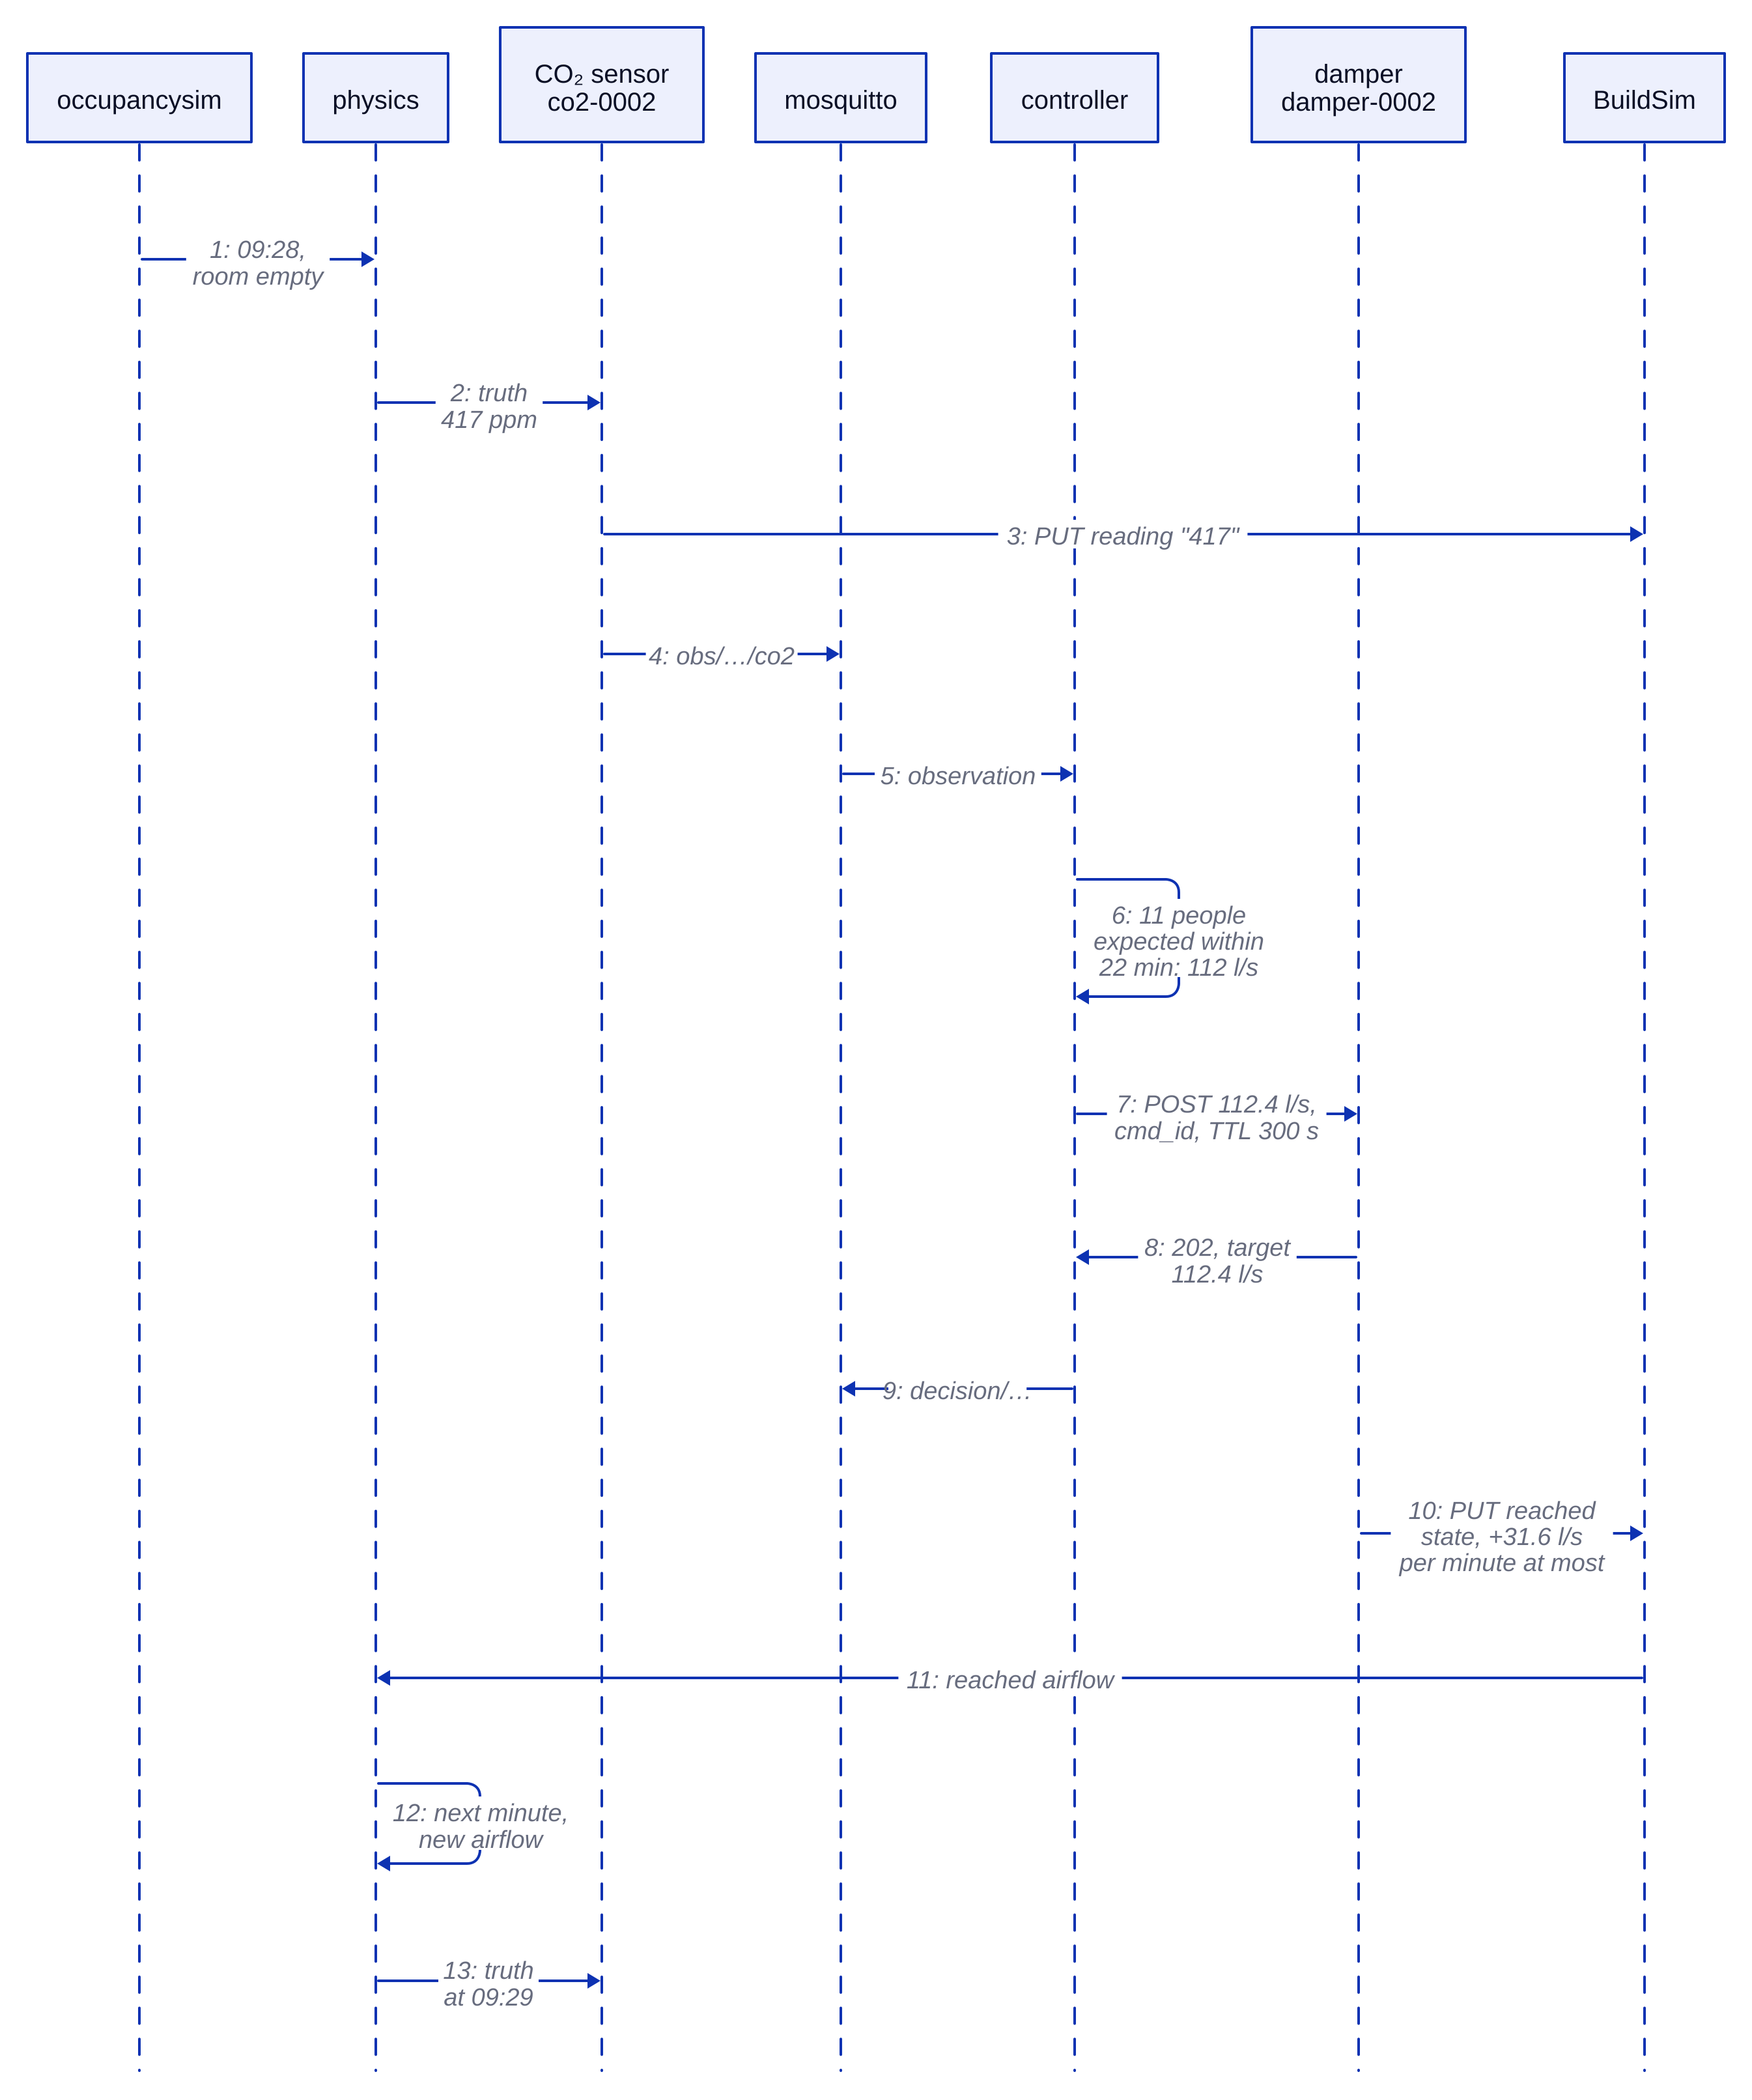
\includegraphics[width=\linewidth]{figures/dynamic.png}
\caption{One control period in fika room 1570 under the predictive policy, at
09:28, about twenty minutes before the morning break. The numbers are from a
run of 2026-09-30.}
\label{fig:dynamic}
\end{figure}

The room is empty and its air is clean, so the reactive term asks for the
minimum. What raises the airflow is step 6: the profile says that about 11
people are usually here within the room's lead time of 22 minutes, and the
workplace rule gives $7\times 11 + 0.35\times 101 = 112$~l/s for them. The
command (step 7) carries an id, the model time of the reading it was decided
on, and a time to live. The damper answers at once with the target it accepted
(step 8) and then travels towards it at no more than a tenth of its maximum
per model minute, writing each state it reaches to BuildSim (step 10). Physics
reads that state on its next tick (step 11), and from the next model minute
the room is computed with more air (step 12). When the people arrive at about
09:45 the damper is already open.

Three properties of this sequence matter for failures:
\begin{itemize}
\tightlist
\item Steps 3 and 4 are two writes. If the broker is down, step 3 still
  happens, and the controller and the damper find the reading in BuildSim.
\item Step 8 is synchronous. The controller knows whether its command was
  accepted, clamped or refused before it records the decision in step 9.
\item Nothing after step 7 needs the controller. If it dies there, the damper
  carries the command out and holds it for 300~s, then returns to design flow.
\end{itemize}

\subsection{8.2 Process lifecycle: a damper actuator}

\begin{figure}[H]
\centering
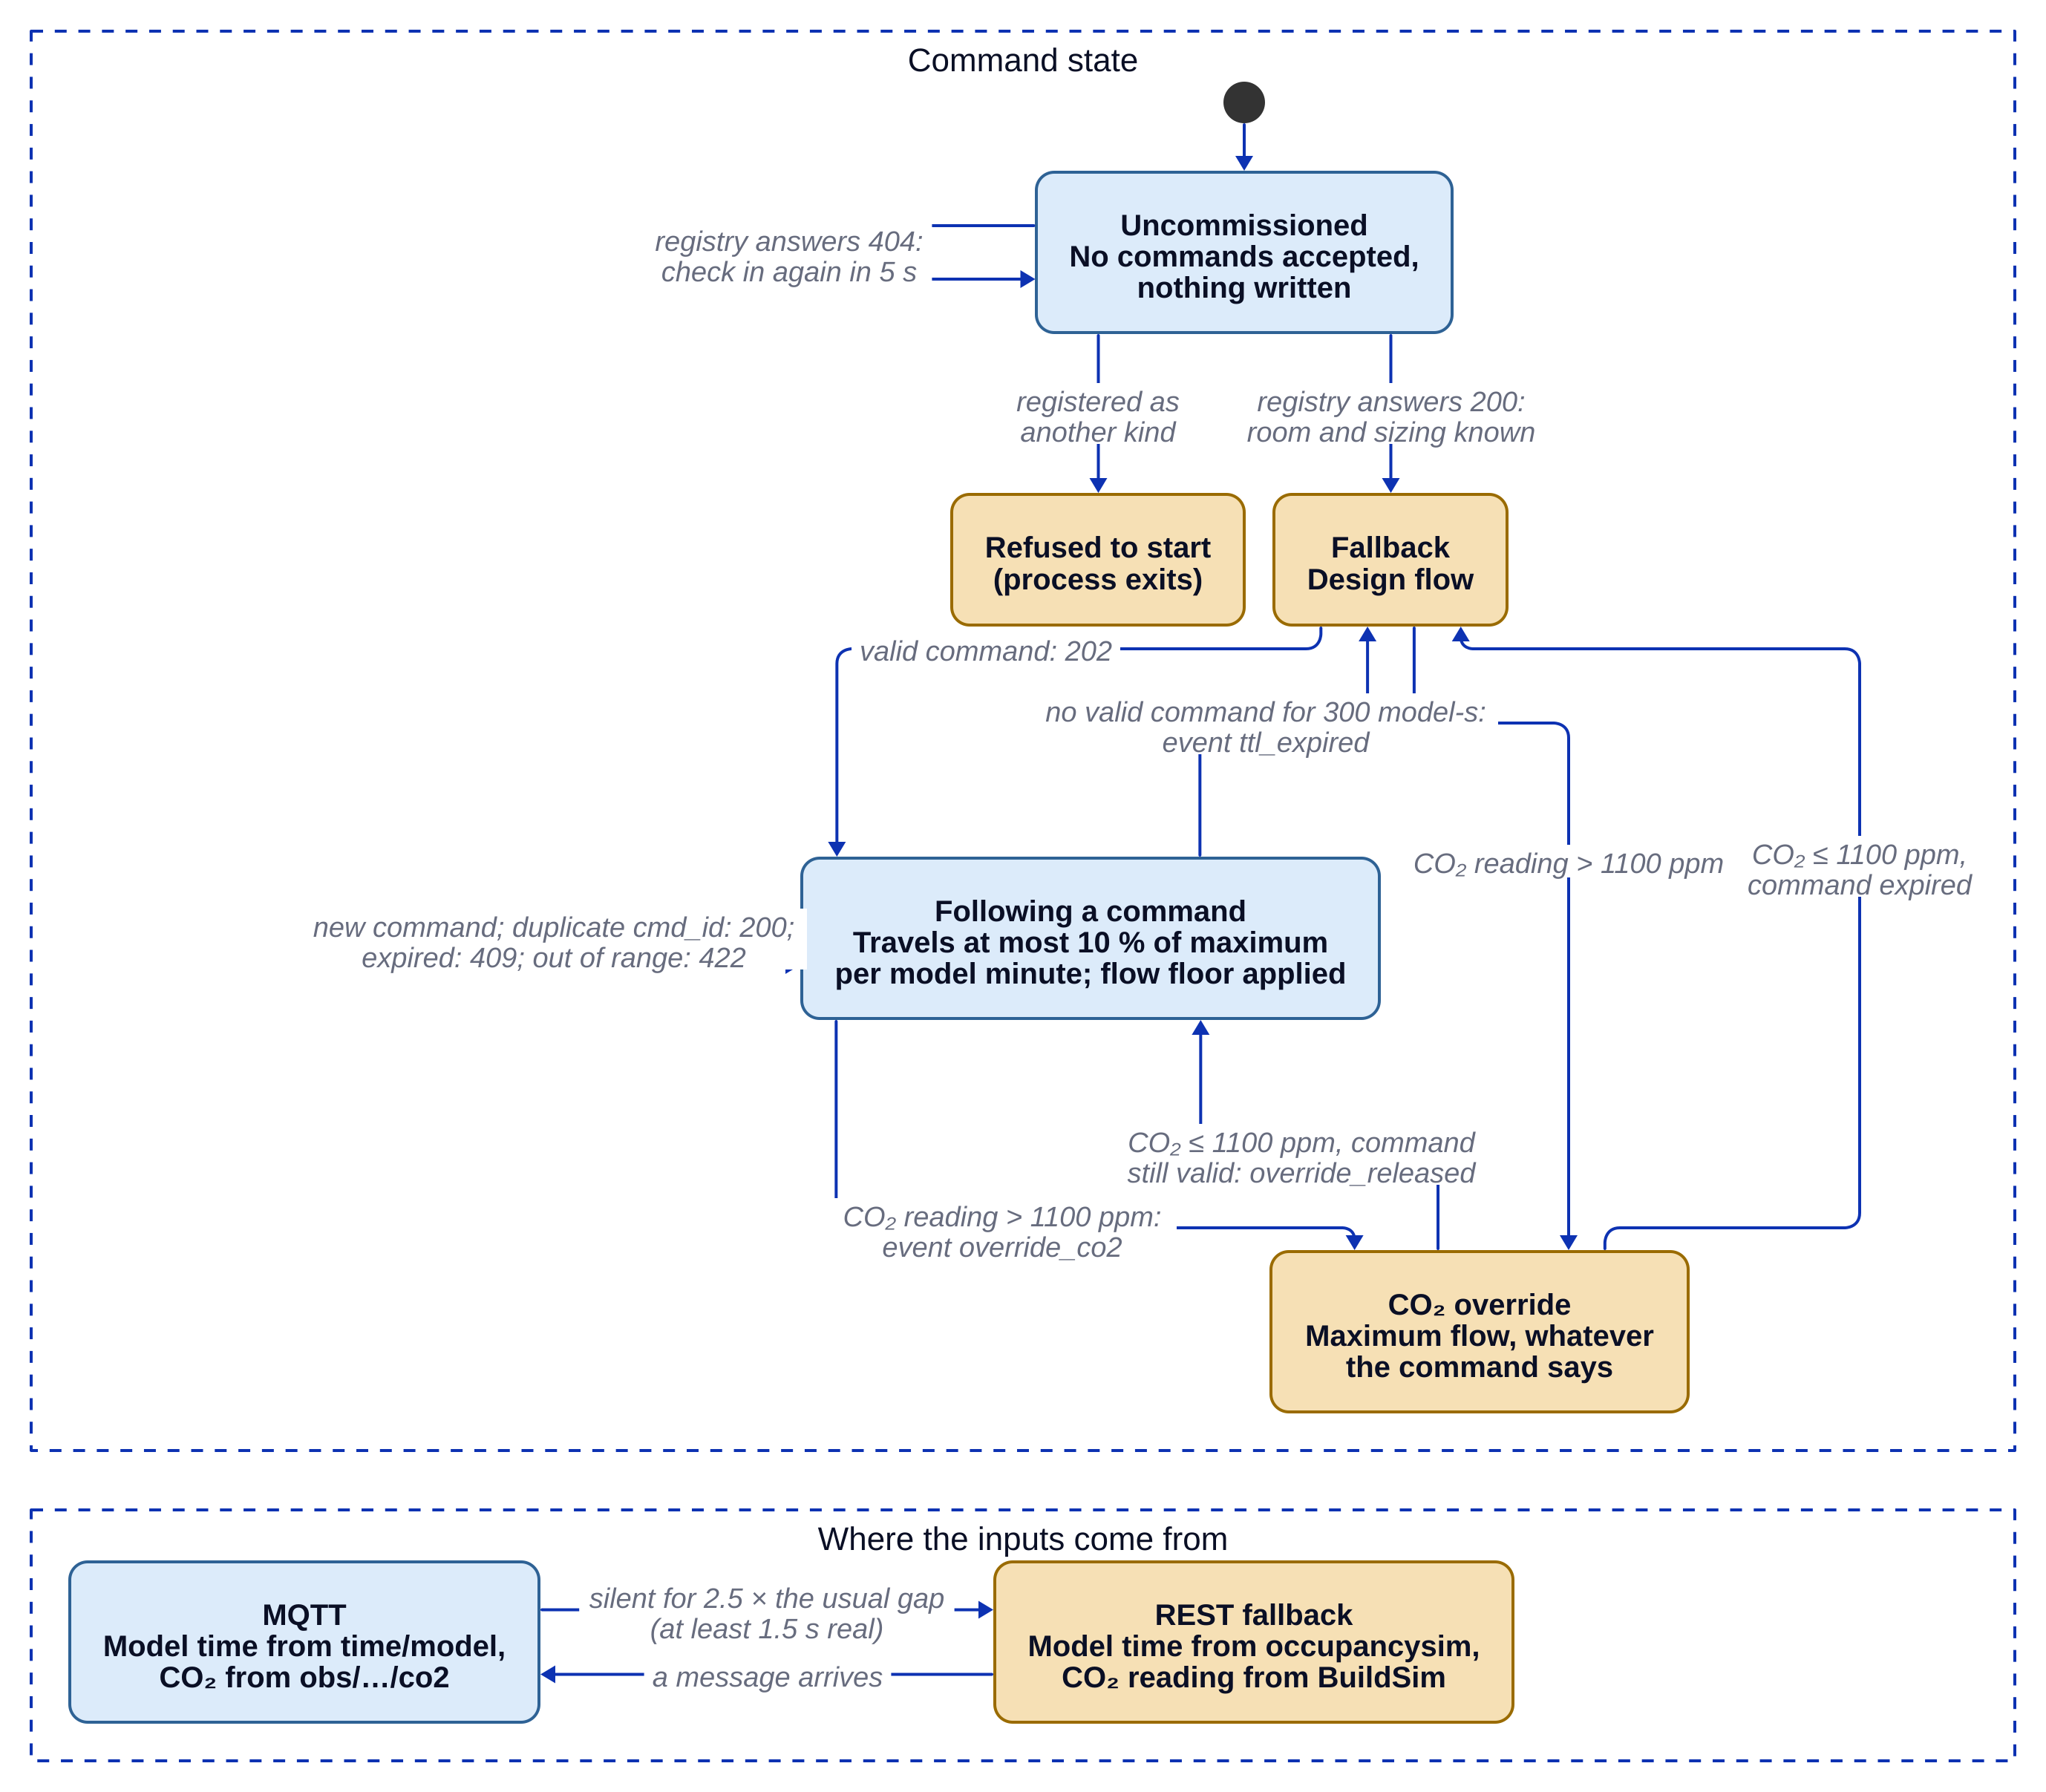
\includegraphics[width=0.86\linewidth]{figures/state.png}
\caption{States of one damper actuator. Blue states are normal operation,
yellow ones are fallbacks. A radiator valve is the same without the override,
and its fallback is 21~°C.}
\label{fig:state}
\end{figure}

\textbf{Start-up.} A device knows only its id and what kind of hardware it is.
It asks the registry every 5~s real until an installer has registered it, and
does nothing else in the meantime. If the registry says it is another kind of
device, it refuses to start, so a mistyped entry cannot make a damper act as a
valve. Once it knows its room and the room's sizing it starts in the fallback,
at design flow.

\textbf{Commands.} A valid command moves it to \emph{following}. Each further
command is checked again. If none arrives for the command's time to live, the
actuator publishes \code{ttl\_expired} and returns to the fallback. This one
transition covers a dead controller, a silent \COtwo{} sensor and a lost
network path between them, without the actuator having to tell them apart.

\textbf{Override.} From either state, a \COtwo{} reading above 1100~ppm opens
the damper fully and publishes \code{override\_co2}. Commands are still
received and remembered during an override, but the target stays at the
maximum until a reading is back at or below 1100~ppm.

\textbf{When the network drops.} The actuator takes the model time and the
room's \COtwo{} from the broker. If either goes silent, for 2.5 times the usual
gap between messages and at least 1.5~s real, it asks occupancysim for the
time and BuildSim for the reading instead, and returns to the broker as soon as
a message arrives. Without any source of time it keeps its current target and
cannot expire a command; that is the one situation in which a stale command
outlives its time to live. If BuildSim restarts, the actuator's writes are
refused until the registry has recreated its equipment, at most 10~s real, and
then continue.

The command, fallback and override transitions are branches in
\code{internal/actuator}, each with a unit test (T-07 to T-11). The start-up
transitions are covered by the commissioning tests (T-28 to T-31).

\section{9. Deployment and component placement}

\begin{figure}[H]
\centering
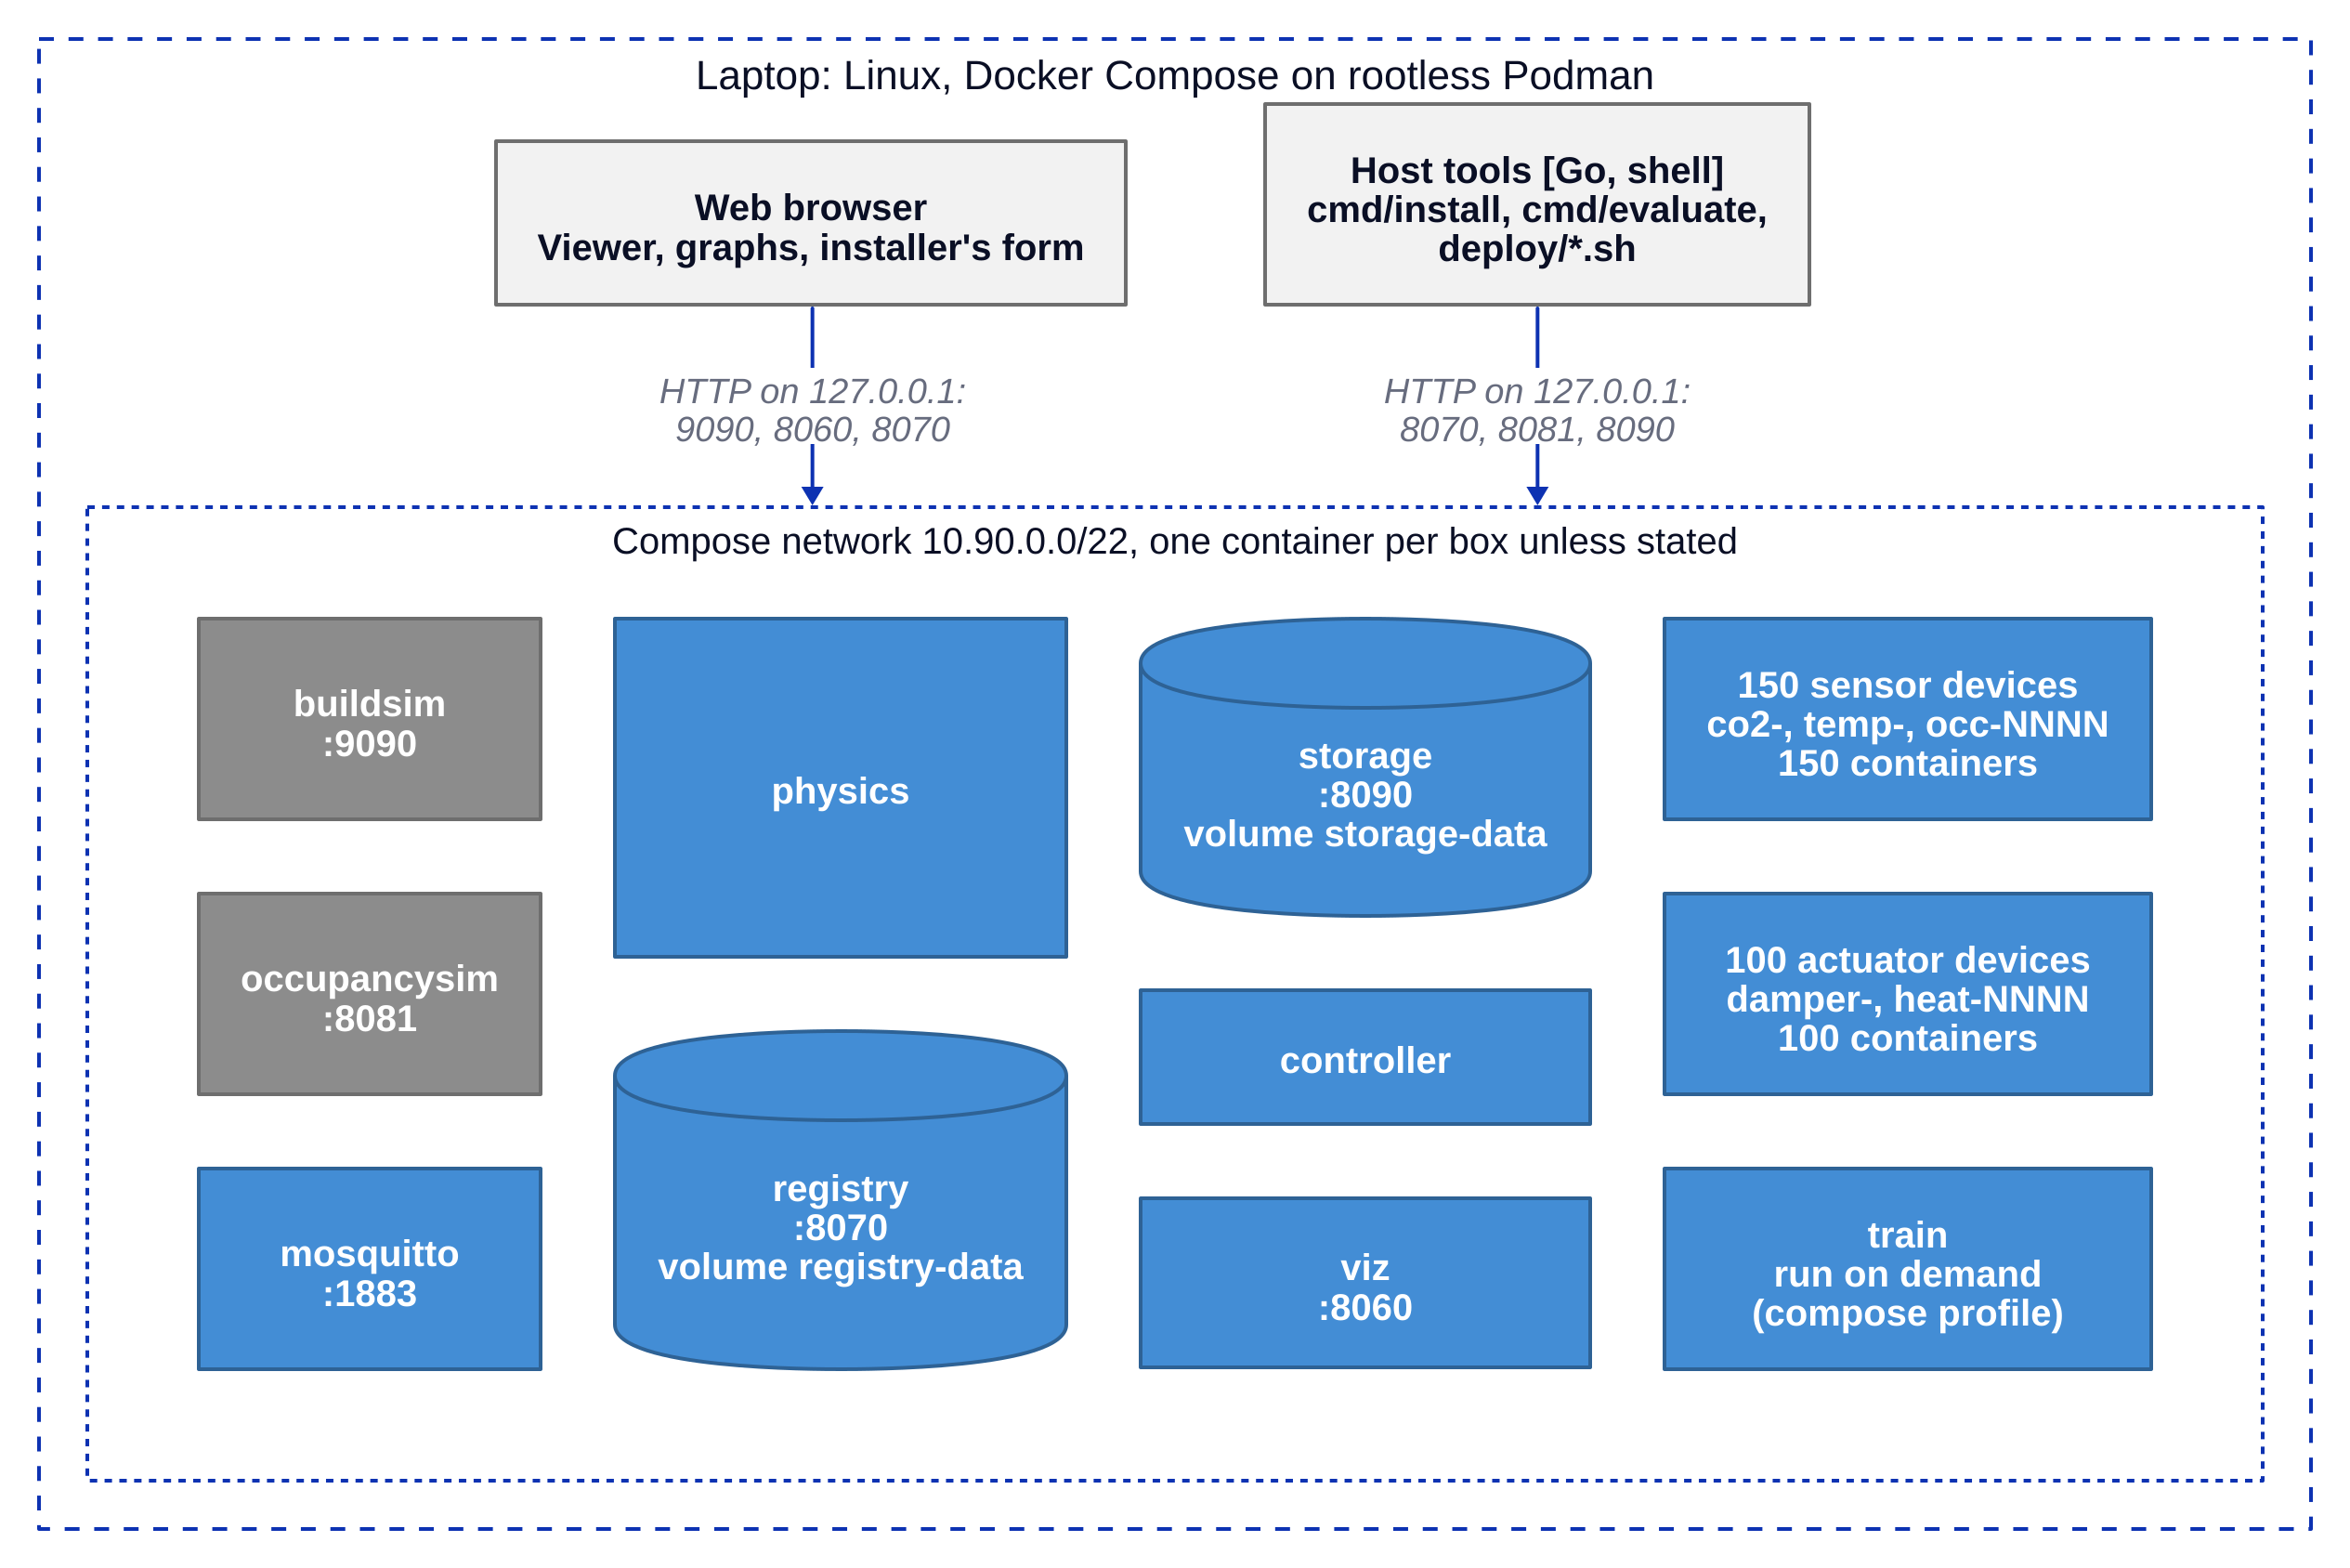
\includegraphics[width=0.86\linewidth]{figures/deployment.png}
\caption{Deployment. Everything runs on one laptop; the links between the
containers are those of Figures~\ref{fig:container}
and~\ref{fig:container-support}. Ports are published on 127.0.0.1 only.}
\label{fig:deployment}
\end{figure}

Everything runs on one laptop, as 258 containers under Docker Compose: the 8
services of \code{compose.yaml} and the 250 devices of the generated
\code{compose.devices.yaml}. Deployment is therefore about how the system is
cut into processes and what each cut buys, not about geography.

\textbf{Isolation.} Each container has one job and talks to the others only
through the interfaces of Section 5. No two share memory or files; the only
volumes are the registry's database and storage's run files, each used by one
container. A container can be stopped, started and replaced on its own, which
is what the fault tests of Section 10 do.

\textbf{Where each part would run in a real building.} The cut into containers
follows that question:
\begin{itemize}
\tightlist
\item \textbf{Sensor and actuator devices} are the hardware in the rooms. That
  is why they are one process each, why the safety limits live in the
  actuator, and why a device learns its room from a registry and not from a
  configuration file.
\item \textbf{The broker, the controller, the registry and storage} belong on
  a server in the building. The control loop must not depend on a connection
  to anywhere else, and a decision per room and minute needs no more than a
  small machine: the whole stack used about one CPU core at factor 60, which
  is sixty times real time.
\item \textbf{Training} is the only part that could move off-site. It is batch
  work, it is off the control path, and if its result never arrives the
  controller keeps the model it has, or runs reactively without one.
\item \textbf{The dashboard} can run anywhere that reaches the broker. It only
  reads.
\item \textbf{physics and occupancysim} would not exist. They stand in for the
  building and its people.
\end{itemize}

\textbf{What merging would cost.} Merging the devices into one process per
kind, which we built first, means one crash silences a kind of sensor in every
room. Merging the safety limits into the controller means they die with it.
Merging storage into the controller means the dashboard and the trainer read
the controller's files, which the course forbids and which ties three
lifetimes together.

\textbf{What one process per device costs.} 250 device containers are the
largest operational cost of the design, and they made the laptop, not our
code, the first limit (Section 11): Podman's keyring per container, the size of
the compose network, and the kernel's neighbour table all had to be raised
before 50 rooms would start. The compose network is a /22 for that reason.
On the development laptop (16 hardware threads) all containers together used
about one core at factor 60, started in about 40~s, and the 250 devices
registered in 26~s (2026-09-30). On a second laptop the same stack used about
1.2 cores and 1.7~GB of memory, started in 90~s and registered in 5~s
(2026-10-10).

\textbf{Operation.} \code{docker compose up -d} starts everything.
Devices start uncommissioned, so the installation list is registered once with
\code{cmd/install}; the registry's database is a volume, so this survives
restarts. \code{RUN\_ID} tags every record of an experiment and is set for the
whole stack at once. The policy is changed by restarting the controller alone.

\section{10. Test plan}

\subsection{10.1 How the system is tested}

Tests are at five levels, and each requirement is verified at the lowest level
that can show it.
\begin{itemize}
\tightlist
\item \textbf{Unit} (\code{go test ./...}, no network): 79 tests in 18 files.
  All logic that decides something is in a package without I/O, so it can be
  tested this way: the room model, the sensor noise, the actuator's rules, the
  policies, the predictor, the stuck-sensor detector, the dashboard's state,
  storage's validation. All pass at commit \code{e9b01be} (run 2026-10-10).
\item \textbf{Integration}: the containers under Docker Compose, with all 50
  rooms.
\item \textbf{Fault}: a fault injected on purpose into the running stack. The
  sensor-fault tests are one scripted run, \code{deploy/fault-tests.sh}, in
  which each fault goes in at a fixed model time with the clock paused, on a
  day that occupancysim generates the same every time.
\item \textbf{Performance}: counts of what arrived and what was dropped,
  under load.
\item \textbf{Evaluation}: full runs of five simulated weekdays per policy
  (Section 11).
\end{itemize}

\textbf{Evidence} comes from the same place for every level above unit: the
run's records in storage. Every reading, true state, decision and actuator
event is stored with its model time and run id, so a test's result is a query
on a named run, and can be repeated by anyone with the run's export. The full
list of 39 test cases, with the observed result of each, is in
\code{docs/test-plan.md}; the table below is its summary by requirement.

\subsection{10.2 Requirements, tests and results}

\begin{longtable}[]{@{}L{0.07\linewidth}L{0.25\linewidth}L{0.44\linewidth}L{0.13\linewidth}@{}}
\toprule
\textbf{Req.} & \textbf{Test} & \textbf{Evidence} & \textbf{Result} \\
\midrule
\endhead
FR-1 & T-01 step response; T-02 clock jump of 3~h (unit) &
\COtwo{} reaches 63~\% of its rise at $t=\tau$ within 5~\%; the jump is cut into
one-minute steps, no overshoot & Met \\
FR-2 & T-03 noise statistics over 10\,000 samples; T-04 fault modes (unit) &
Mean error about 0 and the configured spread for each kind; each fault gives
its signal and leaves other sensors alone & Met \\
FR-3 & T-05 one room end to end (integration) & Run \code{scale50-reactive-3}:
21\,392 of 21\,400 commands accepted over 184 minutes, the 8 others at a manual
clock jump. In T-39 the graphs show a damper's commanded step and its
rate-limited ramp behind it. The four policies give different \COtwo{} for
identical occupancy (Section 11), which an open loop could not & Met \\
FR-4 & T-06 forecast against ``same as now'' on the held-out week; T-35
training on noisy counts (unit) & Fika rooms: 86.7~\% of arrivals foreseen,
against none. But mean absolute error is \emph{higher} than ``same as now'' in
fika rooms (4.23 against 2.33) and lecture rooms (1.13 against 0.81), lower
only in offices (0.60 against 0.64) & \textbf{Not met as stated} (Section 11.3) \\
FR-5 & T-07 validation; T-08 travel rate (unit) & 422, 422, 409 and
200-duplicate, state unchanged in all four; reached state rises by at most
10~\% of maximum per minute & Met \\
FR-6 & T-09 override (unit, and live with a drifting sensor); T-11 flow floors
(unit); T-10 override with the controller killed & Unit: maximum flow above
1100~ppm, release below, floors of 0.35 and 0.10~l/s·m² applied. Live
2026-10-08: reading passed 1100~ppm, damper at 100~\%, critical alert, cleared
with the fault. T-10 has no recorded run & Met, except T-10 \\
FR-7 & T-12 stuck counter; T-13 silent \COtwo{} sensor; T-36 stuck \COtwo{}
and temperature sensors (fault); T-37 detector alone (unit); T-38 detector
replayed over the evaluation runs & Section 10.3. No false alarm in 4.3
million checks on fault-free runs & Met, with the blind spots of Section 13 \\
FR-8 & T-14 rebuild a result from a run's export & Every table in Section 11
is generated by \code{cmd/evaluate} from storage alone. Rebuilding one from
the exported tar has not been done & Partly \\
FR-9 & T-32 policies differ only where they should (unit); T-15 configuration
diff of two runs & Unit test passes. \code{deploy/evaluate.sh} passes only the
run id, the policy and the oracle's source run. The four runs' true occupancy
is identical in all 360\,500 shared records. The diff itself is not recorded &
Met by construction \\
FR-10 & T-16 layers and alerts; T-39 graphs (unit, and live with 50 rooms) &
Five layers with all 50 rooms; a stopped sensor leaves the layer and raises
two alerts that clear on its return; graphs continue after a restart of viz
(9.9 million records re-read in 49~s) & Met \\
FR-11 & T-17 BuildSim restart; T-28 unregistered device; T-29 installer
mistakes; T-30 retirement; T-31 wrong kind & 2026-09-30: equipment of all five
devices restored in under 15~s; an unregistered device stays silent and
starts once registered; a mistyped room is rejected (\code{422}); a retired
device stops at its next check-in. T-31 has no recorded run & Met, except T-31 \\
NFR-1 & T-18 & \code{predictive}: 100.0~\% of occupied room-minutes at or below
1000~ppm, peak 972~ppm & Met \\
NFR-2 & T-19 & 100.0~\% within 20--24~°C under every policy & Met \\
NFR-3 & T-20 & \code{predictive} uses 74~\% less than \code{constant}, and
3.8~\% \emph{more} than \code{reactive}, for 0 against 4 occupied minutes above
1000~ppm & First half met; second half \textbf{not met} \\
NFR-4 & T-21 command latency & Not measured: no record carries the real time
at which a command was sent or a state written & \textbf{Not verified} \\
NFR-5 & T-22 load & 50 rooms at factor 60: 50 of 50 readings of every kind in
every one of 184 minutes. At factor 120: 4 of 10\,500 \COtwo{} readings missed.
No run with more than 50 rooms (Section 11.5) & Met at 50 rooms \\
NFR-6 & T-13, T-17, T-24, T-39 (single failures); T-23 kill each container in
turn & Sensor stopped, broker stopped, BuildSim restarted, viz restarted: each
degrades as designed and recovers (Section 10.3). Killing the controller,
storage, physics, the registry or an actuator has no recorded run &
Partly verified \\
NFR-7 & T-25 same day at factor 600 and at factor 120, truth compared record
by record & 39\,200 truth records in common, no difference in head-count,
guards, \COtwo{} or temperature & Met \\
NFR-8 & T-26 & Each evaluation run of five weekdays took about one hour at
factor 120 & Met \\
\bottomrule
\end{longtable}

\todo{Before submission, either run the tests that have no recorded result or
say here that they were not run: T-10 and T-23 (stop the controller, storage,
physics, the registry and one actuator in turn during a run, and check the
dampers' fallback and the recovery time), T-31, T-14, T-15. T-17 was expected
within 10~s and recorded as ``under 15~s'': re-measure or change the
expectation. For NFR-4, either add a real-time stamp to the decision record
and the actuator's write and measure it, or keep ``not verified''.}

\subsection{10.3 Fault injection: what was observed}

All from run \code{fault-tests} of 2026-10-08 unless another run is named.

\begin{longtable}[]{@{}L{0.20\linewidth}L{0.72\linewidth}@{}}
\toprule
\textbf{Fault} & \textbf{Observed} \\
\midrule
\endhead
\COtwo{} sensor stuck (T-36, room 1570) & Frozen at 425~ppm at 09:30, found at
09:34 after five identical readings. All 47 decisions until the repair at
10:20 command the design flow of 210~l/s. Up to 12 people were in the room
while the sensor said 425; the true \COtwo{} peaked at 571~ppm \\
Temperature sensor stuck (T-36) & Frozen at 07:45, found at 07:56, setpoint
held at 21~°C, normal again at 08:16 \\
\COtwo{} sensor silent (T-13, room 1543) & Stopped at 08:30. Last airflow
decision 08:30; \code{ttl\_expired} at 08:35; the damper travelled from 54~l/s
to the design 600~l/s by 08:45. Heating decisions went on throughout. Both
alerts cleared when the sensor returned at 08:50 \\
People counter stuck (T-12, room A1519) & Frozen at 53 at 11:00 with 53 people
in the room. Not blamed during the hour the lecture went on. The room emptied
at 12:01 and the damper stayed at 408~l/s for ``53 people''; found at 12:16,
flow down to the 37~l/s floor by 12:25; normal two minutes after the repair at
12:40 \\
People counter stuck on a small number (earlier run) & Frozen at 4 in a
25-person room: never found in three hours. Four people's \COtwo{} at full flow
is inside the sensor noise. This is the detector's documented blind spot \\
Broker stopped (T-24, 2026-09-30) & The controller fell back to polling
BuildSim after 4~s real and returned to MQTT when the broker did; no command
expired. Storage recorded nothing for about 20 minutes: the gap is reported,
not filled. The first attempt failed this test: the fallback waited 5~s real,
which at factor 60 is longer than the command's time to live then in use. The
wait now adapts to the message rate, and the time to live is 300~s \\
BuildSim restarted (T-17, 2026-09-30) & It came back blank; the registry
recreated the devices' equipment and readings resumed \\
Dashboard restarted (T-39, 2026-10-09) & viz re-read the run so far from
storage and the graphs continued; the airflow reached before the restart is
not recovered \\
Drifting \COtwo{} sensor (2026-10-08) & Not detected as a fault. The reading
passes 1100~ppm and the damper's override opens it fully: wasteful, but the
safe side \\
\bottomrule
\end{longtable}

\section{11. Evaluation and results}

\subsection{11.1 Setup}

Four policies were run over the same simulated week, after a training week
that the predictor learned from. Every table in this section is generated by
\code{cmd/evaluate} from the stored records of the runs named here.

\begin{longtable}[]{@{}L{0.16\linewidth}L{0.76\linewidth}@{}}
\toprule
\endhead
\textbf{Building} & 50 rooms on the ground floor: 3 fika rooms, 20 lecture rooms, 24 offices and 3 unused rooms; 5 devices each \\
\textbf{Training} & Run \code{train-week-v2}: reactive policy, Mon 14 to Fri 18 Sep 2026, factor 120; 360\,000 people-counter readings; model \code{profile-train-week-v3} \\
\textbf{Evaluation} & Mon 21 to Fri 25 Sep 2026, held out from training, factor 120. Runs \code{eval-constant-v2}, \code{eval-reactive-v2}, \code{eval-predictive-v3} and \code{eval-oracle-v2}, which replays the true occupancy of \code{eval-reactive-v2} \\
\textbf{Fairness} & Same rooms, devices and dates; physics starts every run from fresh rooms; only the policy differs. Verified: all four runs have the same head-count and guard count in every one of 360\,500 shared truth records \\
\textbf{Heating} & The same in every run: schedule with optimal start \\
\textbf{Occupied} & A room counts as occupied when someone other than a guard on patrol is in it. The 481 guard-only records per run are counted separately \\
\textbf{Data} & One truth record per room and model minute, 7\,211 minutes, about 2.16 million records per run, none rejected by storage. At least 99.9~\% of sensor readings of every kind arrived \\
\bottomrule
\end{longtable}

\subsection{11.2 Air quality, comfort and energy}

\begin{longtable}[]{@{}L{0.36\linewidth}L{0.13\linewidth}L{0.13\linewidth}L{0.13\linewidth}L{0.13\linewidth}@{}}
\toprule
 & \textbf{Constant} & \textbf{Reactive} & \textbf{Predictive} & \textbf{Oracle} \\
\midrule
\endhead
\COtwo{} at or below 1000 ppm, occupied (NFR-1: at least 95~\%) & 95.5~\% & 100.0~\% & 100.0~\% & 100.0~\% \\
\quad in lecture rooms only & 65.2~\% & 100.0~\% & 100.0~\% & 100.0~\% \\
Occupied room-minutes above 1000 ppm & 612 & 4 & 0 & 0 \\
Peak \COtwo{} & 1084 ppm & 1024 ppm & 972 ppm & 968 ppm \\
20--24 °C, occupied (NFR-2: at least 95~\%) & 100.0~\% & 100.0~\% & 100.0~\% & 100.0~\% \\
Energy over the week & 25\,285 kWh & 6\,282 kWh & 6\,521 kWh & 6\,370 kWh \\
Saving against constant (NFR-3: at least 30~\%) & & 75~\% & 74~\% & 75~\% \\
Energy against reactive & +302~\% & & +3.8~\% & +1.4~\% \\
\bottomrule
\end{longtable}

\begin{figure}[H]
\centering
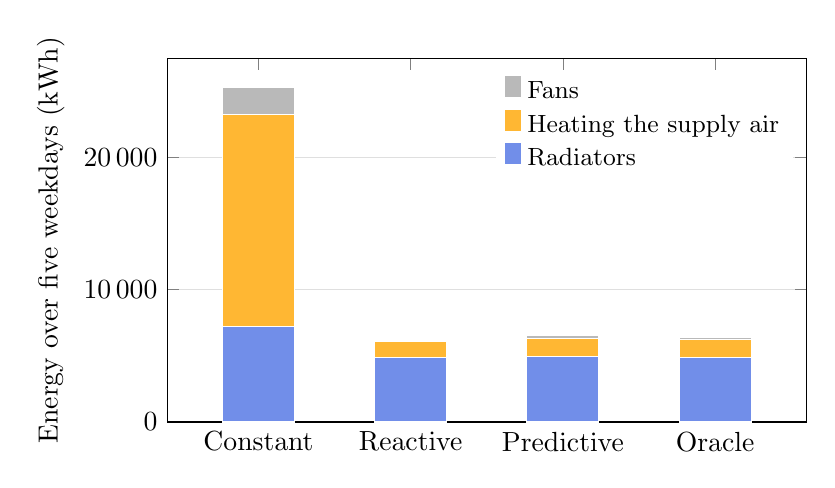
\begin{tikzpicture}
\begin{axis}[
  ybar stacked, width=0.80\linewidth, height=6.2cm, bar width=26pt,
  ymin=0, ymax=27500, enlarge x limits=0.2,
  ylabel={Energy over five weekdays (kWh)},
  symbolic x coords={Constant,Reactive,Predictive,Oracle}, xtick=data,
  scaled y ticks=false, yticklabel style={/pgf/number format/fixed,/pgf/number format/1000 sep={\,}},
  ymajorgrids, grid style={gray!25},
  legend style={at={(0.98,0.97)},anchor=north east,draw=none,font=\small},
  legend cell align=left, reverse legend]
\addplot+[fill=RoyalBlue!75,draw=white] coordinates {(Constant,7224) (Reactive,4892) (Predictive,4933) (Oracle,4908)};
\addplot+[fill=Orange!80,draw=white] coordinates {(Constant,16055) (Reactive,1235) (Predictive,1412) (Oracle,1300)};
\addplot+[fill=gray!55,draw=white] coordinates {(Constant,2007) (Reactive,154) (Predictive,176) (Oracle,162)};
\legend{Radiators,Heating the supply air,Fans}
\end{axis}
\end{tikzpicture}
\caption{The energy proxy by part. Almost all of the difference between
constant flow and the other policies is the heating of supply air that nobody
needed. The three demand-controlled policies differ by a few per cent.}
\label{fig:energy}
\end{figure}

\textbf{Constant ventilation is expensive and still not good enough.} Design
flow day and night costs four times the energy of the other policies, and full
lecture rooms still exceed 1000~ppm in a third of their occupied minutes. That
is what the sizing table in Section 6 predicts: a full room at design flow
settles right around the limit.

\textbf{Reactive control already does almost all of it.} It meets NFR-1 with
four minutes above 1000~ppm all week, in fika rooms, at the lowest energy.

\textbf{Anticipation buys a little, for a little.} With perfect knowledge of
the future, the oracle removes those four minutes and lowers the peak from
1024 to 968~ppm, for 1.4~\% more energy. Because the four runs saw exactly the
same week, that 1.4~\% is a real difference and not noise. The proposal said
that a small gap between reactive control and the oracle would be a result
worth reporting; here it is. The likely reasons are in the design, not the
policy: a damper reaches 1.5 times design flow within a few minutes, and a
lecture room at design flow has a time constant of 12 minutes, so a reactive
controller catches up fast.

\textbf{The predictor gets the oracle's air quality for 3.8~\% more energy
than reactive.} No occupied minute above 1000~ppm, peak 972~ppm. The 2.4~\% it
spends beyond the oracle is the price of an imperfect forecast: it ventilates
fika rooms for a break on days when the break turns out small, and it reacts
to the counter's occasional false ``one person''. This is where the second
half of NFR-3 fails: \code{predictive} was required to use no more energy than
\code{reactive}, and it uses 3.8~\% more. With these rooms and dampers the
honest conclusion is that reactive control is the better trade unless the last
four minutes above the limit matter.

\textbf{Comfort is met everywhere}, now that heating starts before 07:00.

\missingfigure{Response over time: measured \COtwo{}, people counted and
airflow in fika room 1570 on one morning of the evaluation week, 09:00 to
11:00, for \code{reactive}, \code{predictive} and \code{oracle}. The data is in
the storage volume on the PC that ran the evaluation: storage's
\code{/history} with \code{run=eval-predictive-v3}, \code{room=level0/1570}
and \code, and the same for the other two runs.}

\subsection{11.3 The forecast}

Model \code{profile-train-week-v3} on the held-out run \code{eval-reactive-v2},
at every people-counter reading on weekdays 07--18: the peak count within the
next 20 minutes, against the forecast and against ``same as now''. An arrival
is a rise of at least 5 people within the 20 minutes.

\begin{longtable}[]{@{}L{0.10\linewidth}L{0.11\linewidth}L{0.12\linewidth}L{0.14\linewidth}L{0.10\linewidth}L{0.10\linewidth}L{0.11\linewidth}@{}}
\toprule
\textbf{Role} & \textbf{Readings} & \textbf{Forecast MAE} & \textbf{``Same as now'' MAE} & \textbf{Arrivals} & \textbf{Foreseen} & \textbf{False alarms} \\
\midrule
\endhead
Fika & 9\,900 & 4.23 & 2.33 & 1\,042 & 86.7~\% & 22.6~\% \\
Lecture & 65\,920 & 1.13 & 0.81 & 283 & 0.0~\% & 1.1~\% \\
Office & 79\,122 & 0.60 & 0.64 & 0 & & 0.0~\% \\
\bottomrule
\end{longtable}

\textbf{FR-4 is not met as we wrote it.} The requirement asked for a lower
error than ``same as now'', and by mean absolute error the forecast is worse
in fika and lecture rooms. The measure was badly chosen: the forecast is a high
quantile on purpose, so it overshoots most of the time by design, and ``same as
now'' is right whenever nothing changes, which is most minutes. What the
controller needs from a forecast is warning of an arrival, and there the
picture is the opposite: the forecast foresees 87~\% of the arrivals in fika
rooms, with a false alarm in 23~\% of quiet moments, and ``same as now''
foresees none by definition.

\textbf{It warns ahead of fika breaks, but not of lectures.} In lecture rooms
the forecast foresaw none of 283 arrivals. occupancysim puts each lecture in a
random room every slot and day, so a single room has no pattern to learn, and
no model trained on that room's history could do better. A timetable as an
input would fix it.

\textbf{More data made the model worse.} The first model trained on a reading
per minute expected at least one person in about 86~\% of all 15-minute slots
in every room, nights included, and the predictive run that used it spent
25~\% more energy than reactive, most of it on empty rooms. The cause was how
the training treated the counter's noise. The counter shows one person too many
in about 5~\% of readings. The training took the \emph{highest} reading of each
slot and day, and with 15 readings per slot an empty room shows a false ``1''
on more than half of the days ($1 - 0.95^{15} = 54~\%$). The earlier, thinner
training data had three readings per slot, and the same flaw touched about
15~\% of slots without being noticed. The predictor's unit tests used
noise-free data and passed.

\begin{longtable}[]{@{}L{0.40\linewidth}L{0.13\linewidth}L{0.11\linewidth}L{0.10\linewidth}L{0.10\linewidth}@{}}
\toprule
 & \textbf{Before the fix} & \textbf{After} & \textbf{Reactive} & \textbf{Oracle} \\
\midrule
\endhead
Slots at night in which the model expects someone & 82--88~\% & 0~\% & & \\
Mean airflow in empty rooms at night & 30.9 l/s & 8.7 l/s & 7.5 l/s & 7.7 l/s \\
Mean airflow in empty rooms, 09--17 & 35.1 l/s & 28.3 l/s & 25.8 l/s & 26.6 l/s \\
Energy over the week & 7\,877 kWh & 6\,521 kWh & 6\,282 kWh & 6\,370 kWh \\
Energy against reactive & +25~\% & +3.8~\% & & +1.4~\% \\
Fika arrivals foreseen / false alarms & 97 / 25~\% & 87 / 23~\% & & \\
\bottomrule
\end{longtable}

The fix takes the 75th percentile of a slot's readings and counts a forecast
below half a person as an empty room. The model was retrained on the same
stored week and only the predictive run repeated
(\code{eval-predictive-v2} is kept as the evidence for the flaw). A regression
test now trains on a week of noisy readings from an empty room (T-35). That
only one run had to be repeated is the reproducibility work of D-1 paying off:
the other three runs do not use the model, and the weeks are identical.

\subsection{11.4 What the first evaluation changed}

A first evaluation on 2026-10-01 exposed three things that were fixed before
the runs above.

\begin{longtable}[]{@{}L{0.26\linewidth}L{0.38\linewidth}L{0.28\linewidth}@{}}
\toprule
\textbf{Finding} & \textbf{Cause} & \textbf{Fix and effect} \\
\midrule
\endhead
Comfort only 96--97~\%; 84--88~\% in lecture rooms & Heating switched to 21~°C at 07:00 sharp: rooms were at 17.9~°C and reached 20~°C about 08:13 & Optimal start: rooms at 20.9~°C at 07:00; comfort 100~\%; about 2.5~\% more energy \\
Cold ``occupied'' minutes at night & Guards on patrol counted as occupants of a room in setback & The measure changed, not the heating: a room with only a guard in it is counted as a patrol \\
Runs of the same week agreed in only 99.6--99.7~\% of samples & Each run sampled occupancy through its own coarse window (D-1) & Per-minute record in occupancysim; runs now identical (T-25) \\
\bottomrule
\end{longtable}

The ranking of the policies and the size of the effects did not change between
the two evaluations.

\subsection{11.5 Scale and the breaking point}

\textbf{What 50 rooms cost.} At factor 60, with 150 sensors reporting once per
real second, every reading of every kind arrived in every one of 184 minutes
(run \code{scale50-reactive-3}), and all containers together used about one of
the laptop's 16 hardware threads. At factor 120, which doubles the rate to 300
readings and 200 commands per real second, 4 of 10\,500 \COtwo{} readings were
missed over 210 minutes, the controller dropped none as stale, and storage
rejected none of 63\,792 records (run \code{load120}). NFR-5 holds at 50 rooms.

\textbf{What broke first was the host, not our code.} One container per device
means about five containers per room, and a stock Linux laptop stops at about
200 containers, which is 40 rooms:

\begin{longtable}[]{@{}L{0.30\linewidth}L{0.30\linewidth}L{0.32\linewidth}@{}}
\toprule
\textbf{Limit} & \textbf{Symptom} & \textbf{Fix} \\
\midrule
\endhead
Kernel keyring quota: 200 keys per user, and Podman gives every container a keyring & Only about 195 containers started; the rest failed with ``Disk quota exceeded'' & \code{keyring = false} in the user's Podman configuration \\
The compose network is a /24 by default: 254 addresses & ``IPAM error: failed to find free IP'' & A /22 in \code{compose.yaml} \\
Kernel neighbour table: 1024 entries, shared by all containers; each holds an entry per peer it talks to & DNS lookups failed, sensors could not reach physics, no readings & Raise the kernel's \code{gc\_thresh} limits (needs root) \\
BuildSim's floor plan took over 2~s under load & 10 of 250 registrations timed out & 15~s for floor-plan reads \\
\bottomrule
\end{longtable}

\textbf{What breaks next is time, not rooms.} A sensor polls physics every
250~ms real, and a model minute lasts 1~s real at factor 60 and 0.5~s at factor
120. As the factor rises, a sensor starts to miss minutes: none at factor 60,
0.01 to 0.10~\% of readings at factor 120. An earlier version that polled once
per real second lost about one reading in five from one sensor at factor 60,
by aliasing with physics' own tick; that is how the polling rate was chosen.
The same design therefore has a ceiling on how much faster than real time it
can be evaluated, which matters for evaluation cost and not for a real
building, where the factor is 1.

\todo{The grade-5 test (T-22) asks for the point at which the system stops
working. Two cheap experiments would give it as a measured curve: (a) the
share of readings that arrive at factors 60, 120, 240, 480 and 600 with 50
rooms, two simulated hours each, a few minutes in total; (b) the same at factor
60 with 100 rooms (\code{go run ./cmd/gendevices -plan 100}), if the laptop
starts 500 containers. Replace this note with the plot, or state that no run
beyond 50 rooms was made.}

\subsection{11.6 Where the numbers are weak}

\begin{itemize}
\tightlist
\item \textbf{The building is a model we wrote.} With slower dampers or a
  smaller maximum flow, the gap between reactive control and the oracle would
  be wider. The result says as much about the model's time constants as about
  the controllers.
\item \textbf{One seed, one week.} A second seed would show how stable the
  ranking is. The 1.4~\% and 3.8~\% differences are exact for this week and
  untested for any other.
\item \textbf{The control loop's timing is not reproducible}, by design: when
  a reading arrives and when a command lands depend on separate processes. The
  occupancy each policy faces is identical; the exact timing of its commands
  is not.
\item \textbf{The predictive run is two days newer} than the other three, with
  the predictor's fix in between. That is sound only because the simulated
  week is identical in all four, which was verified record by record.
\item \textbf{The stuck-sensor detector was added after the runs.} Replaying
  the runs' readings through it gave no verdict (T-38), so no decision would
  have differed.
\item \textbf{The heating's warm-up rate is assumed}, and rooms are warm about
  an hour before 07:00. That energy is in every policy's total.
\item \textbf{Command latency was not measured} (NFR-4).
\end{itemize}

\section{12. Dashboard}

The dashboard is one process, \code{viz}, with two faces. It builds both from
what the control system itself sees: the observations, the decisions and the
actuator events on MQTT. The true state of the rooms is not on any topic it may
read, so the dashboard shows what was measured, never what was true.

\subsection{12.1 The building now: layers and alerts in the BuildSim viewer}

viz writes five room layers to BuildSim once per real second, and the 3D viewer
colours each room by the layer chosen. The viewer itself is provided by the
course; what is ours is what is mapped into it.

\begin{longtable}[]{@{}L{0.24\linewidth}L{0.18\linewidth}L{0.16\linewidth}L{0.32\linewidth}@{}}
\toprule
\textbf{Layer} & \textbf{Source} & \textbf{Range} & \textbf{Colours} \\
\midrule
\endhead
\COtwo{} & sensor reading & 400--1600 ppm & Blue to red around grey at the 1000~ppm limit \\
People counted & sensor reading & 0--50 & Light to dark blue \\
People expected soon & prediction & 0--50 & Light to dark blue \\
Airflow & actuator state & 0--100~\% of the room's maximum & Light to dark blue \\
Temperature & sensor reading & 17--27 °C & Blue to red around grey at 22~°C \\
\bottomrule
\end{longtable}

A quantity of ``how much'' is one hue from light to dark; a quantity on either
side of a target is blue and red around a neutral grey that sits exactly on the
target. Airflow is shown as a share of each room's own maximum, because an
office's 20~l/s and a lecture room's 900~l/s do not fit one scale. A room drops
out of a layer when its reading is more than 180~s old or its sensor has been
found stuck: either colour would claim something nobody measured.

Alerts are the current picture, at most 100, most severe first:

\begin{longtable}[]{@{}L{0.11\linewidth}L{0.36\linewidth}L{0.22\linewidth}L{0.21\linewidth}@{}}
\toprule
\textbf{Severity} & \textbf{Alert} & \textbf{Raised by} & \textbf{Cleared by} \\
\midrule
\endhead
Critical & \COtwo{} override in a room & event \code{override\_co2} & \code{override\_released} \\
Warning & No reading from a room's sensor & a reading older than 180~s & its next reading \\
Warning & A sensor looks stuck, with what was seen and what the system does about it & a decision with a \code{fault} & the next decision without one \\
Warning & Damper or radiator valve on fallback & event \code{ttl\_expired} & the next accepted command \\
Warning & Command rejected & event \code{rejected} & five minutes later \\
Info & No trained model, once for the building & decisions in mode \code{no\_forecast} & normal decisions \\
\bottomrule
\end{longtable}

\missingfigure{Screenshot of the BuildSim viewer with the \COtwo{} layer and at
least one alert, for example during \code{deploy/fault-tests.sh}:
\code{http://127.0.0.1:9090/?layer=co2\&floor=level0}.}

\subsection{12.2 The building over time: the graphs page}

The viewer answers ``what is the building doing now''. Most of what a
ventilation system is asked is about time: did the air stay good through the
lecture, when did the damper open, what did the fault do. viz therefore serves
its own page, one HTML file with no outside dependencies, so it also works
without internet.

\begin{itemize}
\tightlist
\item \textbf{The building:} people counted, ventilation power and its share
  of what constant flow would use, rooms above the \COtwo{} limit, and alerts;
  three graphs over time; the alert log; a table of every room.
\item \textbf{One room:} \COtwo{} with the limit and the override level; people
  counted and people ventilated for; airflow commanded and reached, with design
  and maximum flow; temperature and setpoint with the comfort band. The times
  an alert was active are shaded in all four.
\item The range is the last hour, 6 hours, 24 hours or 7 days. Pointing at a
  moment in one graph shows it in all of them, by mouse or keyboard, and every
  graph has its values as a table underneath.
\end{itemize}

In every graph blue is what was measured or reached and orange is what the
controller expected or commanded; yellow and red mean an alert and nothing
else. A minute in which nothing was seen is a hole in the line, never a zero
and never the previous value. The one derived number, ventilation power, is
the summed reached airflow times the energy proxy's constants for fans and
supply-air heating; the radiators are left out because their power depends on
the true room temperature, which the dashboard never sees.

The history is held in viz's memory, one point per room and model minute for a
week. Storage remains the owner of the history: after a restart viz reads the
run so far from it, so a killed dashboard comes back with its graphs (T-39).

\missingfigure{Screenshot of the graphs page, room view, showing a fault: for
example room 1570 during the stuck \COtwo{} sensor of T-36 (flat \COtwo{} line,
shaded alert period, the damper's step to design flow).
\code{http://127.0.0.1:8060}.}

What the graphs showed that the tables had not: summed over the building, the
predictive policy's ``people ventilated for'' runs well ahead of the people
counted in the morning (57 against 6 at 09:29 on a development run). That gap
is the extra energy over the reactive policy, as a picture.

\section{13. Risks and critical reflection}

\textbf{The headline result is that the clever part buys little.} The proposal
set out to show that predicting occupancy pays off. It does not, here: reactive
control on \COtwo{} is within four room-minutes per week of perfect foresight,
and our predictor closes that gap for 3.8~\% more energy. We think the finding
is real for this model and would not carry to every building. The dampers reach
maximum flow in minutes and the maximum is 1.5 times design flow, so a
reactive controller is never far behind. A building with slower or smaller
ventilation would show a larger gap. We did not vary those constants, which is
the experiment we would run next.

\textbf{The predictor cannot see what matters most.} The rooms that fill
fastest are the lecture rooms, and they are the ones with no pattern: the
forecast foresaw none of their arrivals. The fix is an input, not a better
model: the day's bookings are available from occupancysim and could be read as
a booking system would provide them. We parked that for time.

\textbf{We measured the forecast with the wrong yardstick.} FR-4 asked for a
lower mean error than ``same as now'', which a deliberately high forecast
cannot give. We report it as not met and say what should have been asked:
arrivals foreseen at a stated false-alarm rate.

\textbf{What changed from the proposal, and what it cost.} The proposal's main
claim was occupancy without an occupancy sensor. We gave each room a people
counter instead, and the system no longer shows that \COtwo{} alone is enough.
The mass balance we meant to invert is used only as two bounds, to catch a
counter that is stuck. A full estimator would also give the degraded mode a
head-count when the counter fails, which today it replaces with the forecast.

\textbf{Mistakes that the tests did not catch.} Three faults got past the
unit tests: the predictor that learned sensor noise (its tests used clean
data), the runs of one day that were not identical (we had written ``same
seed'' under fairness without checking), and FR-7, which promised a fallback
for a stuck sensor that nothing detected. The first two were found by looking
at evaluation results that seemed implausible, the third by re-reading what we
had promised while writing the alerts. None was found by a failing test. Each
now has a regression test or a recorded run.

\begin{longtable}[]{@{}L{0.30\linewidth}L{0.28\linewidth}L{0.34\linewidth}@{}}
\toprule
\textbf{Risk or assumption} & \textbf{Impact} & \textbf{Mitigation, or decision} \\
\midrule
\endhead
The room physics is our own model, with assumed constants & Energy and comfort figures say as much about the model as about the controllers & Reported as comparisons between policies on the same model, never as absolute savings \\
A drifting sensor is not detected & A \COtwo{} sensor drifting up ends in the override: safe, wasteful. One drifting down would be believed & Not solved. Cross-checking neighbouring rooms, or the counter against \COtwo{}, is the next step \\
A people counter stuck on a small number is not found & Seen live: stuck at 4 in a 25-person room for three hours & Accepted: it costs the airflow for four people. Pinned by a unit test so the limit is known \\
A stuck counter is found only after the air disagrees & 15--20 minutes in a lecture room, about 75 in an office & Accepted; the cost is airflow, not air quality \\
The stuck-sensor limits come from our own noise model & A real sensor quieter than its resolution repeats itself when healthy and would be blamed & The limits would have to be set from the real sensor's noise at commissioning \\
The truth API is closed to the controller by convention only & The controller could call physics; it has no code that does & The truth \emph{topic} is enforced by the broker. A separate network for the truth layer would close the rest \\
Devices do not authenticate to the registry & Any process on the network can pose as a device & A real installation would give each device a secret at commissioning \\
The broker is a single point for observations & Decisions continue through the BuildSim fallback, but storage records nothing while it is down & Accepted and reported: a 20-minute gap in T-24 \\
The live count reacts to one false reading & About 5~\% of the predictive policy's decisions in an empty room ventilate for ``one person'' & Requiring two readings would remove it, at a minute's delay for a real first arrival. Not done \\
Command latency was never measured & NFR-4 is unverified & Records carry model time only; a real-time stamp is needed first \\
One seed and one week & The ranking of the policies is untested on other weeks & A second seed is five more hours of runs \\
250 containers on one laptop & A stock laptop stops at about 40 rooms; with three host settings raised, 50 run. More was not tried & One process per device is right for a real installation and expensive to simulate \\
The heating's warm-up rate is assumed & Rooms are warm about an hour early & Learning the rate per room from earlier mornings \\
\bottomrule
\end{longtable}

\textbf{How the design was reviewed.} We used an AI assistant throughout, and
kept a log of where its advice was wrong and how we caught it
(\code{docs/review-log.md}). The pattern is worth stating: its first designs
were plausible and broke rules it had not been shown. It put the sensor noise
inside physics, shared files between processes and showed true \COtwo{} in the
viewer, all three against the lectures; it treated occupancysim as something
we could not change; and it proposed the stuck-counter rule that blames every
healthy counter. Each was caught by checking the design against the course
material or by asking what a healthy system looks like, before or after code
was written. The parts of this design we are most sure of are the ones that
were wrong once.

\todo{Decide whether the paragraph above belongs in the report, and check
what Canvas says about declaring AI use. This draft was itself written with
the assistant, from your documents.}

\textbf{With more time.} In order: vary the damper and room constants to see
when anticipation starts to pay; give the predictor the timetable; measure
command latency; a second seed; drift detection; and the \COtwo{}-based
occupancy estimate the proposal started from.


\end{document}
